\documentclass[aps,prb,twocolumn,superscriptaddress,amsmath,amssymb,floatfix]{revtex4}
%\documentclass[aps,prb,onecolumn,preprint,superscriptaddress,amsmath,amssymb,floatfix]{revtex4}
%\documentclass[aps,prl,onecolumn,groupedaddress,amsmath,amssymb,12pt]{revtex4}
\usepackage{graphicx}
\usepackage{ifthen}
\usepackage{dcolumn}% Align table columns on decimal point
\usepackage{bm}% bold math
\usepackage{multirow}
\usepackage{booktabs}
\usepackage{amsbsy}
\usepackage{amsmath}
\usepackage{amssymb}
\usepackage{subfigure}


%Definition of new commands
\newcommand{\f}[2]{\ensuremath{\frac{\displaystyle{#1}}{\displaystyle{#2}}}}
\newcommand{\lr}[1]{\langle{#1}\rangle}
\newcommand{\colv}[2] {\left(\begin{array}{c} #1 \\ #2 \end{array}\right)}
\renewcommand{\thefootnote}{\fnsymbol{footnote}}
\newcommand{\be} {\begin{eqnarray}}
\newcommand{\ee} {\end{eqnarray}}
%--------------------------------------------------------------------------
%EQ COMMANDS
%--------------------------------------------------------------------------
\newcommand{\two}{\mspace{-2.0mu}}
\newcommand{\four}{\mspace{-4.0mu}}
\newcommand{\plus}{\mspace{-4.5mu}+\mspace{-3.5mu}}
\newcommand{\minus}{\mspace{-4.5mu}-\mspace{-3.5mu}}
\newcommand{\pp}{'\mspace{-2.0mu}'}
\newcommand{\xlb}[4]{#1\ifthenelse{\equal{#2}{0}}{}{_{\alpha #2}}
\mspace{-2.0mu}\genfrac{(}{)}{0pt}{1}{\ifthenelse{\equal{#3}{0}}{0}{l #3}} 
{\ifthenelse{\equal{#4}{0}}{0}{b #4}}}

\newcommand{\xkv}[4]{#1\mspace{-5.0mu}\left(\mspace{-8.0mu}
\begin{smallmatrix}#2\four{}\four{}\mspace{-8.0mu}&\pmb{\kappa}#3\\&\nu 
#4\end{smallmatrix}\mspace{-5.0mu}\right)}

\newcommand{\evect}[6]{#1\mspace{-4.0mu}\left(\mspace{-8.0mu}
\begin{smallmatrix}#2\mspace{-8.0mu}&\pmb{\kappa} #3 &b #5\\&\nu #4 &
\alpha #6\end{smallmatrix}\mspace{-5.0mu}\right)}

\newcommand{\varmat}[8]{\mspace{-5.0mu}\left(\mspace{-8.0mu}
\begin{smallmatrix}\ifthenelse{\equal{#3}{0}}{\mspace{-8.0mu}&b_{#1}&b_{#2}
\\&\alpha_{#1}&\alpha_{#2}} {\ifthenelse{\equal{#7}{0}}{#1\mspace{-8.0mu}&
\pmb{\kappa}#2#3\mspace{-8.0mu}&\pmb{\kappa}#4#5\mspace{-8.0mu}&\pmb{\kappa}
#6\\&\nu#2&\nu#4&\nu#6} {#1\mspace{-8.0mu}&\pmb{\kappa}#2#3\mspace{-8.0mu}&
\pmb{\kappa}#4#5\mspace{-8.0mu}&\pmb{\kappa}#6#7\mspace{-8.0mu}&\pmb{\kappa}
#8\\&\nu#2&\nu#4&\nu#6&\nu#8}}\end{smallmatrix}\mspace{-5.0mu}\right)}

\newcommand{\EXP}[1]{\exp\mspace{-5.0mu}\left[#1\right]\mspace{-3.0mu}}

\newcommand{\tpp}[2]{\left(\mspace{-2.0mu}\xkv{\omega}{}{}{}#1\xkv{\omega}
{}{'}{'}#2\xkv{\omega}{}{\pp}{\pp}\mspace{-2.0mu}\right)}



%--------------------------------------------------------------------------
\newcommand{\SUM}[2]{\ifthenelse{\equal{#1}{0}}{\sum_{
\alpha_{#2},b_{#2},l_{#2}}^{3,n,N}} {\ifthenelse{\equal{#1}{1}}{\sum_{
\alpha_{#2},b_{#2}}^{3,n}}{\sum_{\pmb{\kappa}#2,\nu#2}^{N,3n}}}}

\newcommand{\SUMprime}[2]{\ifthenelse{\equal{#1}{0}}
{\sum_{\alpha_{#2},b_{#2},l_{#2}}^{3,n,N}} 
{\ifthenelse{\equal{#1}{1}}{\sum_{\alpha_{#2},b_{#2}}^{3,n}}
{\sum_{\pmb{\kappa}^{'}#2,\nu#2}^{N,3n}}}}

\newcommand{\SUMalpha}[2]{\ifthenelse{\equal{#1}{0}}
{\sum_{\alpha_{#2}}^{3}} {\ifthenelse{\equal{#1}{1}}
{\sum_{\alpha_{#2},b_{#2}}^{3,n}}{\sum_{\pmb{\kappa}#2,\nu#2}^{N,3n}}}}
%--------------------------------------------------------------------------
\newcommand{\SUMalphap}[2]{\ifthenelse{\equal{#1}{0}}
{\sum_{\alpha'_{#2}}^{3}} {\ifthenelse{\equal{#1}{1}}
{\sum_{\alpha'_{#2},b'_{#2}}^{3,n}}{\sum_{\pmb{\kappa}#2,\nu#2}^{N,3n}}}}

\newcommand{\SUMb}[2]{\ifthenelse{\equal{#1}{0}}{\sum_{b_{#2}}^{n}}
 {\ifthenelse{\equal{#1}{1}}{\sum_{\alpha_{#2},b_{#2}}^{3,n}}
{\sum_{\pmb{\kappa}#2,\nu#2}^{N,3n}}}}

\newcommand{\SUMbp}[2]{\ifthenelse{\equal{#1}{0}}{\sum_{b'_{#2}}^{n}}
 {\ifthenelse{\equal{#1}{1}}{\sum_{\alpha'_{#2},b'_{#2}}^{3,n}}
{\sum_{\pmb{\kappa}#2,\nu#2}^{N,3n}}}}

\newcommand{\SUMl}[2]{\ifthenelse{\equal{#1}{0}}{\sum_{l_{#2}}^{N}}
 {\ifthenelse{\equal{#1}{1}}{\sum_{\alpha_{#2},b_{#2}}^{3,n}}
{\sum_{\pmb{\kappa}#2,\nu#2}^{N,3n}}}}

\newcommand{\SUMlp}[2]{\ifthenelse{\equal{#1}{0}}{\sum_{l'_{#2}}^{N}}
 {\ifthenelse{\equal{#1}{1}}{\sum_{\alpha'_{#2},b'_{#2}}^{3,n}}
{\sum_{\pmb{\kappa}#2,\nu#2}^{N,3n}}}}

\newcommand{\abcdt}[5]{\mspace{-4.0mu}\left(\mspace{-8.0mu}
\begin{smallmatrix}&\ifthenelse{\equal{#1}{}}{a}{#1}&\ifthenelse
{\equal{#3}{}}{c}{#3}\\&\ifthenelse{\equal{#2}{}}{b}{#2}&\ifthenelse
{\equal{#4}{}}{d}{#4}\end{smallmatrix}\mspace{-2.0mu};\ifthenelse
{\equal{#5}{}}{t}{#5}\right)}

\newcommand{\abcd}[4]{\mspace{-4.0mu}\left(\mspace{-8.0mu}
\begin{smallmatrix}&\ifthenelse{\equal{#1}{}}{a}{#1}&\ifthenelse
{\equal{#3}{}}{c}{#3}\\&\ifthenelse{\equal{#2}{}}{b}{#2}&\ifthenelse
{\equal{#4}{}}{d}{#4}\end{smallmatrix}\mspace{-3.0mu}\right)}

\newcommand{\abt}[3]{\mspace{-4.0mu}\left(\mspace{-8.0mu}\begin
{smallmatrix}&\ifthenelse{\equal{#1}{}}{a}{#1} \\&\ifthenelse{
\equal{#2}{}}{b}{#2}\end{smallmatrix}\mspace{-2.0mu};
\ifthenelse{\equal{#3}{}}{t}{#3}\right)}

\newcommand{\ab}[2]{\mspace{-4.0mu}\left(\mspace{-8.0mu}
\begin{smallmatrix}&\ifthenelse{\equal{#1}{}}{a}{#1} \\&\ifthenelse
{\equal{#2}{}}{b}{#2}\end{smallmatrix}\mspace{-3.0mu}\right)}

\newcommand{\kvbat}{\mspace{-4.0mu}\left(\mspace{-8.0mu}
\begin{smallmatrix} &\pmb{\kappa} &b \\ &\nu &\alpha\end{smallmatrix}
\mspace{-2.0mu};t\right)}
%--------------------------------------------------------------------------
\newcommand{\kvbatp}{\mspace{-4.0mu}\left(\mspace{-8.0mu}
\begin{smallmatrix} &\pmb{\kappa} &b' \\ &\nu &\alpha'\end{smallmatrix}
\mspace{-2.0mu};t\right)}

\newcommand{\kvbaw}{\mspace{-4.0mu}\left(\mspace{-8.0mu}
\begin{smallmatrix} &\pmb{\kappa} &b \\ &\nu &\alpha\end{smallmatrix}
\mspace{-2.0mu};\omega\right)}

\newcommand{\kvbawp}{\mspace{-4.0mu}\left(\mspace{-8.0mu}
\begin{smallmatrix} &\pmb{\kappa} &b' \\ &\nu &\alpha'\end{smallmatrix}
\mspace{-2.0mu};\omega\right)}

\newcommand{\kvba}{\mspace{-4.0mu}\left(\mspace{-8.0mu}
\begin{smallmatrix} &\pmb{\kappa} &b \\ &\nu &\alpha\end{smallmatrix}
\mspace{-3.0mu}\right)}

\newcommand{\kvbap}{\mspace{-4.0mu}\left(\mspace{-8.0mu}
\begin{smallmatrix} &\pmb{\kappa}' &b \\ &\nu' &\alpha\end{smallmatrix}
\mspace{-3.0mu}\right)}
%--------------------------------------------------------------------------
\newcommand{\kpvba}{\mspace{-4.0mu}\left(\mspace{-8.0mu}
\begin{smallmatrix} &\pmb{\kappa}^{'} &b \\ &\nu &\alpha\end{smallmatrix}
\mspace{-3.0mu}\right)}

\newcommand{\kva}{\mspace{-4.0mu}\left(\mspace{-8.0mu}
\begin{smallmatrix} &\pmb{\kappa} \\ &\nu &\alpha\end{smallmatrix}
\mspace{-3.0mu}\right)}

\newcommand{\kvap}{\mspace{-4.0mu}\left(\mspace{-8.0mu}
\begin{smallmatrix} &\pmb{\kappa} \\ &\nu &\alpha'\end{smallmatrix}
\mspace{-3.0mu}\right)}

\newcommand{\kvb}{\mspace{-4.0mu}\left(\mspace{-8.0mu}
\begin{smallmatrix} &\pmb{\kappa} &b \\ &\nu \end{smallmatrix}
\mspace{-3.0mu}\right)}

\newcommand{\kvbp}{\mspace{-4.0mu}\left(\mspace{-8.0mu}
\begin{smallmatrix} &\pmb{\kappa} &b' \\ &\nu \end{smallmatrix}
\mspace{-3.0mu}\right)}

\newcommand{\kvt}{\mspace{-4.0mu}\left(\mspace{-8.0mu}
\begin{smallmatrix}&\pmb{\kappa} \\&\nu\end{smallmatrix}
\mspace{-2.0mu};t\right)}

\newcommand{\kvzero}{\mspace{-4.0mu}\left(\mspace{-8.0mu}
\begin{smallmatrix}&\pmb{\kappa} \\&\nu\end{smallmatrix}
\mspace{-2.0mu};0\right)}

\newcommand{\kpvt}{\mspace{-4.0mu}\left(\mspace{-8.0mu}
\begin{smallmatrix}&\pmb{\kappa}^{'} \\&\nu\end{smallmatrix}
\mspace{-2.0mu};t\right)}

\newcommand{\kvw}{\mspace{-4.0mu}\left(\mspace{-8.0mu}
\begin{smallmatrix}&\pmb{\kappa} \\&\nu\end{smallmatrix}
\mspace{-2.0mu};\omega\right)}

\newcommand{\kv}{\mspace{-4.0mu}\left(\mspace{-8.0mu}
\begin{smallmatrix}&\pmb{\kappa} \\&\nu\end{smallmatrix}
\mspace{-3.0mu}\right)}

\newcommand{\kvp}{\mspace{-4.0mu}\left(\mspace{-8.0mu}
\begin{smallmatrix}&\pmb{\kappa'} \\&\nu'\end{smallmatrix}
\mspace{-3.0mu}\right)}

\newcommand{\kw}{\mspace{-4.0mu}\left(\mspace{-8.0mu}
\begin{smallmatrix}&\pmb{\kappa} \\&\omega\end{smallmatrix}
\mspace{-3.0mu}\right)}

\newcommand{\kpvp}{\mspace{-4.0mu}\left(\mspace{-8.0mu}
\begin{smallmatrix}&\pmb{\kappa'} \\&\nu'\end{smallmatrix}
\mspace{-3.0mu}\right)}
%--------------------------------------------------------------------------
\newcommand{\lbt}{\mspace{-4.0mu}\left(\mspace{-8.0mu}
\begin{smallmatrix}&l \\&b\end{smallmatrix}\mspace{-2.0mu};t\right)}

\newcommand{\lbtp}{\mspace{-4.0mu}\left(\mspace{-8.0mu}
\begin{smallmatrix}&l' \\&b'\end{smallmatrix}\mspace{-2.0mu};t\right)}

\newcommand{\lt}{\mspace{-4.0mu}\left(\mspace{-8.0mu}
\begin{smallmatrix}&l\end{smallmatrix}\mspace{-2.0mu};t\right)}

\newcommand{\ltp}{\mspace{-4.0mu}\left(\mspace{-8.0mu}
\begin{smallmatrix}&l'\end{smallmatrix}\mspace{-2.0mu};t\right)}

\newcommand{\lb}{\mspace{-4.0mu}\left(\mspace{-8.0mu}
\begin{smallmatrix}&l \\&b\end{smallmatrix}\mspace{-3.0mu}\right)}

\newcommand{\lbp}{\mspace{-4.0mu}\left(\mspace{-8.0mu}
\begin{smallmatrix}&l' \\&b'\end{smallmatrix}\mspace{-3.0mu}\right)}
%--------------------------------------------------------------------------
%COMMANDS
%--------------------------------------------------------------------------

%--------------------------------------------------------------------------
\begin{document}
%--------------------------------------------------------------------------

%--------------------------------------------------------------------------
\title{Evaluation of the Virtual Crystal Approximation for Predicting 
Thermal Conductivity}
%--------------------------------------------------------------------------
\author{Jason M. Larkin}
\affiliation{Department of Mechanical Engineering\\Carnegie Mellon 
University\\Pittsburgh, PA 15213}
\author{A. J. H. McGaughey}
\email{mcgaughey@cmu.edu}
\affiliation{Department of Mechanical Engineering\\
Carnegie Mellon University\\Pittsburgh, PA 15213}
%--------------------------------------------------------------------------

%--------------------------------------------------------------------------
\date{\today}
%--------------------------------------------------------------------------


%--------------------------------------------------------------------------
\begin{abstract}
%--------------------------------------------------------------------------
In this work, the virtual crystal approximation for mass disorder is 
evaluated by examining two model alloy systems: Lennard-Jones argon 
and Stillinger-Weber silicon. In both cases the perfect crystal is 
alloyed with a heavier mass species up to equal concentration and 
phonon properties and thermal conductivity 
are precited. These 
two alloyed systems have different ranges of phonon frequencies, 
lifetimes, and mean free paths.
For Stillinger-Weber silicon, the 
virtual crystal approximation predicts phonon properties and thermal 
conductivity in good agreement with molecular dynamics-based methods. 
For Lennard-Jones argon, the virtual crystal approximation underpredicts 
the high frequency phonon lifetimes, leading to an underpredicting of 
its thermal conductivity. Resolution of these underpredictions is achieved 
by consindering methods which treat the disorder explicitly. 
%--------------------------------------------------------------------------
\end{abstract}
%--------------------------------------------------------------------------


%--------------------------------------------------------------------------
\maketitle
%--------------------------------------------------------------------------
\clearpage
%--------------------------------------------------------------------------
\section{\label{S:Introduction}Introduction}
%--------------------------------------------------------------------------

Predicting the thermal conductivity of disordered lattices dates back to...
In the case of semiconductors, almost all of the heat is conducted by
the vibrational modes of the system. Understanding the mechanisms that lead 
to the scattering of these vibrations is crucial for predicting the 
thermal conductivity of disordered lattices.

To improve the efficiency of thermoelectric devices, 
efforts to reduce thermal conductivity using several techniques, 
including 
micro- and nano-boundary scattering. These techniques often require 
complicated nanostructuring and manufacturing techniques. 
Alloying remains an effective method to reduce the thermal conductivity 
of materials. In particular, for materials with short phonon mean free path 
spectra, alloying is still a potential thermal conductivity reduction 
mechanism where nanostructuring is not.\cite{tian_phonon_2012}

Accurately predicting the thermal conductivity of a dielectric or 
semiconducting material requires the properties of phonons from the entire 
Brillouin zone. Accurate predictions of phonon properties for bulk systems 
can be made with anharmonic lattice dynamics (ALD) theory 
using ab initio 
calculations.\cite{ward_intrinsic_2010,lindsay_thermal_2012,
garg_role_2011,
shiga_microscopic_2012,tian_phonon_2012,
shiomi_thermal_2011,esfarjani_heat_2011}
However, computational costs limit the size of computational cells 
in ab initio calculations to be less than 100 atoms, making it difficult 
to directly incorporate the effects of disorder.
\cite{koker_thermal_2009,bao_first-principles_2012,
lindsay_thermal_2012,tian_phonon_2012,garg_role_2011}

Recently, work using ab-initio calculations, anharmonic 
lattice dynamics (ALD) and the virtual crystal (VC) 
approximation was done to predict phonon mode frequencies, lifetimes and 
group velocities of defected materials with realtively
large\cite{garg_role_2011,lindsay_thermal_2012} 
and 
small\cite{tian_phonon_2012} 
thermal conductivities. 
Under this approximation, the disordered 
crystal is replaced with a perfect “virtual crystal” with properties 
equivalent to an averaging over the disorder (e.g. mass or bond 
strength).\cite{abeles_lattice_1963}
The use of ALD with VC (referred to herein as VC-ALD) bases 
all calculations on a small unit cell with averaged properties and 
treats the effects of intrinsic and disorder scattering as perturbations 
rather than including disorder explicitly.
\cite{abeles_lattice_1963,tamura_isotope_1983,
tian_phonon_2012,lindsay_thermal_2012} 
However, no comprehensive study has been performed 
to assess the applicability of this perturbative approach for a range 
of disorder using multiple predictive methods and test systems.

The goal of this work is to investigate the use of the VC 
approximation for predicting thermal conductivity of disordered 
lattices by a detailed comparison 
of 3 predictive methods: MD-based normal mode 
decomposition (NMD, Section ) and green-kubo (GK, Section \ref{} ), 
and VC-ALD which treats the harmonic and 
anharmonic phonon scattering as perturbations 
(Section \ref{S:From VC-ALD}).  
Two model binary-alloy systems 
(labeled as $m^a_{1-c}m^b_{c}$, Section ) 
with varying concentrations ($c$) of mass defects  
are considered: 
Lennard-Jones (LJ) argon and Stillinger-Weber (SW) silicon. 
In both cases the perfect crystal is 
alloyed with a heavier mass species up to equal 
concentration ($c=0.5$), spanning 
a range of perturbative to heavy disorder. By spanning this range, 
the limits of the perturbative models are examined.

The LJ argon and SW silicon alloyed 
systems have very different ranges of phonon frequencies, 
lifetimes, group velocities and total thermal conductivity. 
For SW silicon, 
VC-ALD predicts thermal conductivity in good agreement with the 
explicitly disordered method GK (Section ). 
For LJ argon, VC-ALD underpredicts 
the high frequency phonon lifetimes, leading to an underpredicting of 
the thermal conductivity when compared to the explicitly disordered 
methods VC-NMD and GK (Section ). 
The different thermal conductivity spectra  
and the breakdown of the perturbative models are examined. Resolution 
of the breakdown is achieved by including the explicit effect of
disorder on the thermal transport of vibrational modes (Section ). Based 
on the effects of explicit disorder, a simple guideline is suggested 
for use with the VC approximation.

not used yet...
Experimental measurements of isotopically pure and Ge-doped 
Si epitaxial layers demonstrate the original theory by Abeles can predict 
thermal conductivity in dilute alloys. Abeles also found good agreement 
with dilute predictions for both experimental measurements of both 
Si-Ge alloys and also (Ga,In)As alloys.\cite{abeles_lattice_1963} However, 
both of these alloy systems have a relatively high thermal conductivities 
(on the order of 1-10 W/m-K at 300 K). However, in the heavily disordered 
system In(As,P) (mass ratio of 3.7) worse agreement with the Abeles theory 
is observed. 

%--------------------------------------------------------------------------
\subsection{\label{S:Virtual Crystal}Virtual Crystal (VC) Approximation}
%--------------------------------------------------------------------------

Abeles first introduced the idea of using a virtual crystal (VC) to 
replace a disordered one, computing the
thermal conductivity of Si/Ge alloys by treating both
disorder and anharmonicity as perturbations.\cite{abeles_lattice_1963} 
Many experimental trends in thermal conductivity 
of a range of materials 
can be explained using the VC approximation.(cite) For example,
the reduced thermal conductivity of Ge versus Si is partly explained 
by both the increased mass and decreased bulk modulus (stiffness) of the 
lattice,(cite) which has the effect of reducing the phonon group 
velocities. The same effect can be seen in alloy systems.(cite)
Sound speeds of alloys: CRC, (Cahill-Pohl).

A complete 
description of the thermal transpot in both perfect crystals and alloys 
requires modeling the intrinsic 
and disordered scattering to calculate phonon lifetimes 
(see Section \ref{S:From VC-ALD}).
Phonon lifetimes can be predicted by treating both the intrinsic 
and disorder scattering using perturbation theory (Section ). 
While the theory which treats phonon defect scattering (Eq. ) 
is valid for
perturbative disorder, its use leads to good agreement with
several experimental and computational results with large disorder.  
Cahill shows that conductivty reduction in dilute 
Ge-doped Si epitaxial layers 
is captured by mass perturbative disorder.
\cite{cahill_thermal_2004,cahill_thermal_2005} 
While the mass disorder was large ($m_{Ge}/m_{Si} = 2.6$),  
the overall disorder strength is dictated by the concentration. 
As little as $6.2\times10^{19} cm^{-3}$ Ge
($g_2 = 3.1\times10^{-3}$, see Section ) 
is enough to reduce the thermal conductivity of 
Si by almost a factor of 2.\cite{cahill_thermal_2004}
Even in the
case of $Ni_{0.55}Pd_{0.45}$, with large mass disorder and 
concentration ($m_{Pd}/m_{Ni} \approx 2$, $g_2=0.078$ Section ), 
good agreement is also seen using a VC approach.
\cite{kamitakahara_vibrations_1974} What is thermal conductivity 
of NiPd alloy versus amorphous phase, what is the HS prediction.

Computational results using the VC approximation 
for high thermal conductivity 
alloys show good to excellent agreement with experimental results
\cite{garg_role_2011,lindsay_thermal_2012}.
Garg used ab initio calculations with VC-ALD   
to predict the thermal conductivity of Si/Ge alloys 
for all concentrations, obtaining excellent agreement with experiment.
\cite{garg_role_2011}  Lindsay and Broido 
found good agreement with VC-ALD and experiment for 
isotopically defected GaN.\cite{lindsay_thermal_2012}  
Isotopically defected GaN and Si/Ge alloys (even for large 
concentrations $c$, Section) have relatively large 
thermal conductivities.(cite) In 
particular, the conductivity of Si/Ge alloys is significantly 
larger than that of the high scatter limit (Section ). 
A detailed study of low thermal conductivity materials 
PbTe\cite{shiga_microscopic_2012} and PbTe/PbSe\cite{tian_phonon_2012} 
made predictions for the perfect systems in fair agreement with 
experiment, where results lack for the alloys. What is the PbTe HS 
prediction. 
Thus, there is a need to examine the perturbative approach of 
VC-ALD for heavily disordered systems. 
The computational studies discussed above were limited to the use 
of VC-ALD because of the computational cost of ab initio calcualtions. 
Computationally cheap empirical potentials can be used to incude 
the effects of disorder explicitly.

Using computationally-cheap empirical potentials for argon 
and silicon\cite{stillinger_computer_1985},  
we study the effects of disorder explicitly. 
Using the VC approximation, 
we perform calculations at different concentations ($c$) 
of mass varying ($m^a_{1-c}m^b_{c}$) binary alloys of Lennard-Jones 
argon and Stillinger-Weber silicon (Section ). We predict 
the phonon mode properties of the VC:  
frequencies (Section ), group velocities (Section ),  
and lifetimes (Section ), and use them to predict thermal
conductivity (Section ). Methods referred to as VC-NMD (Section )
and VC-ALD (Section ) use the VC approximation. Explicit disorder 
is examined using lattice dynamics (LD) calculations 
(Section and ), Allen-Feldman theory (Section ),\cite{allen_thermal_1993} 
and molecular dynamics (MD) simulations 
(Section ). The breakdown of the perturbative VC-ALD method is examined 
(Section ), and a simple correction is suggested by predictions from 
the AF theory (Section ). 

dunno where this belongs. 

While the group 
velocities are necessary to predict the thermal conductivity, 
of particular interest is the phonon mean free path (MFP), 
\begin{equation}\label{EQ:MFP}
\Lambda\kv = |\pmb{v}_{g}| \tau\kv, 
\end{equation}
which is crucial for understanding 
nano and micro-nanostructuring effects.(cite) It is  
correct to regard the mode lifetime $\tau\kv$ as the more 
fundamental quantity is a disordered system,(cite) since there is no 
general way to predict the group velocities of disordered modes.(cite) 
The effect of disorder on mode group velocities is examined in (Section) 
and (Section). 

%--------------------------------------------------------------------------
\begin{figure}
\begin{center}
\mbox{\subfigure{(a)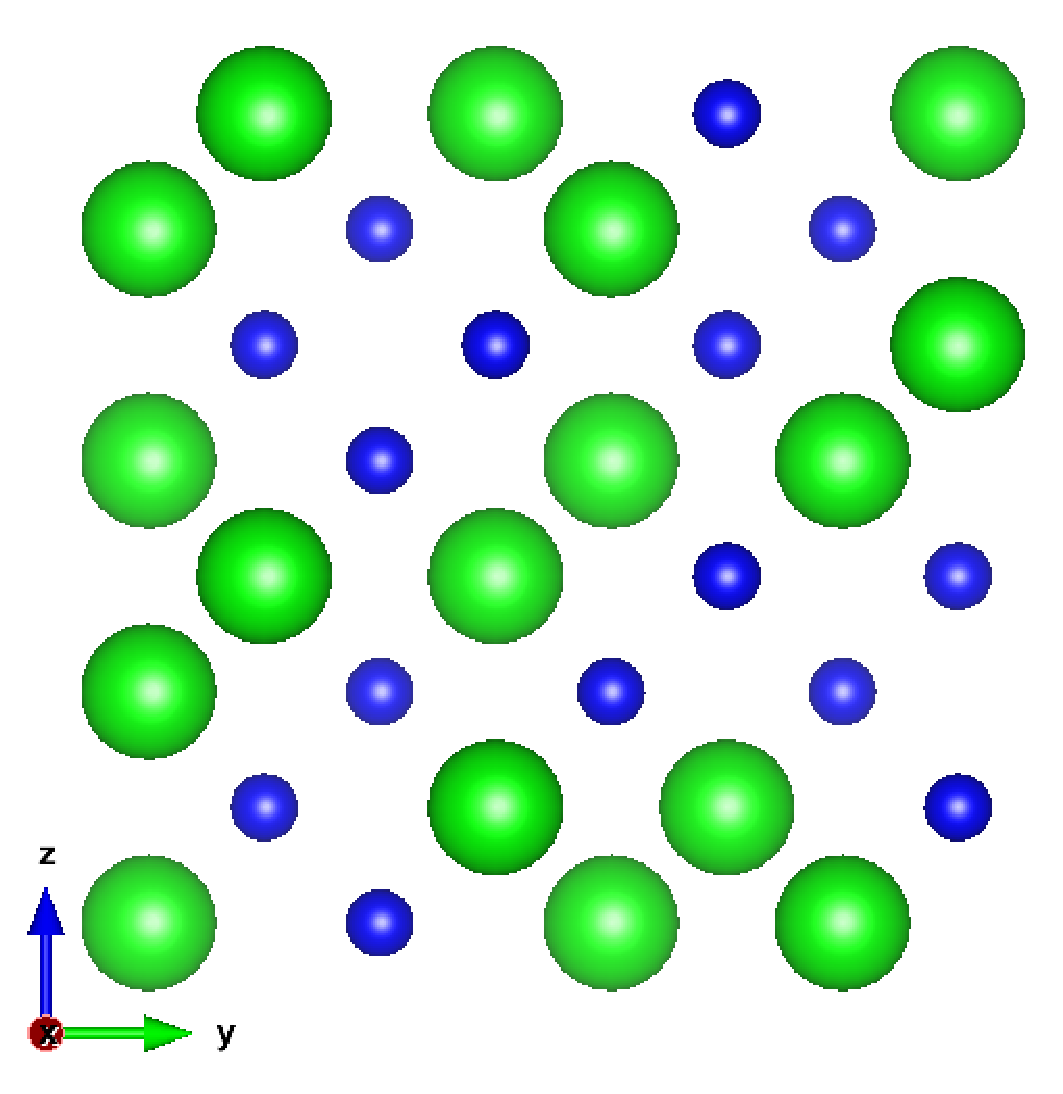
\includegraphics[scale=0.2]
{/home/jason/disorder/si/si_conv_2x2x2_disorder-2.eps}
\subfigure{(b)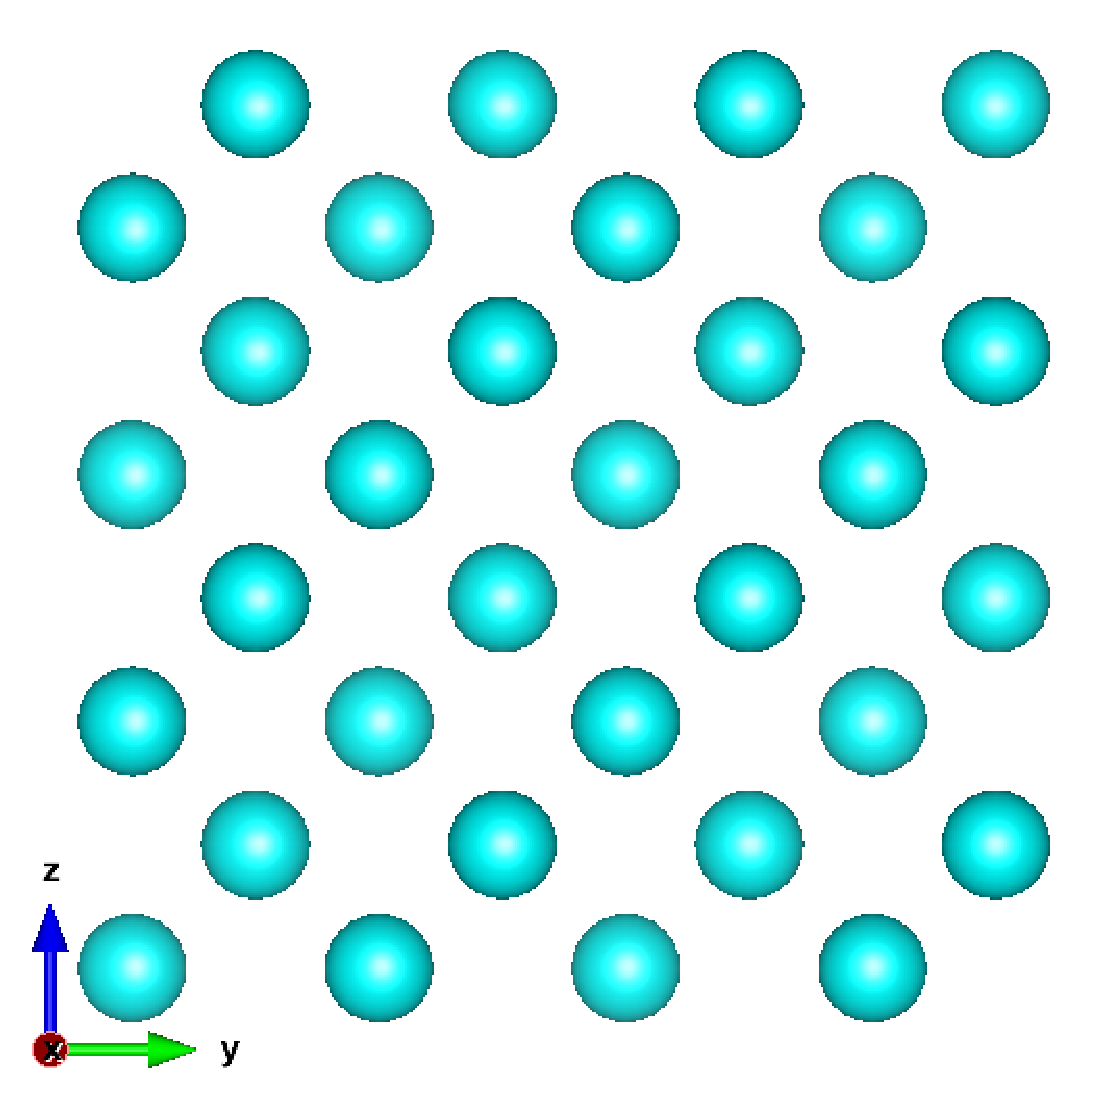
\includegraphics[scale=0.2]
{/home/jason/disorder/si/si_conv_2x2x2_perfect-2.eps}}}}
\vspace*{0mm}
\end{center}
\caption{\label{F:supercells} 
(a) view of an explicitly disoredered supercell of 
Si and ``heavy'' Si ([100] direction into the paper).
\cite{momma_vesta:_2008} 
(b) view of the equivalent VC supercell 
with an average
mass of the explicitly disordered Si and ``heavy'' Si supercell 
(b). 
Sphere size represents 
increasing mass 
only, no bond disorder is considered. 
In this work, calculations for LJ Ar and SW Si which use the VC 
approximation 
are based off of the conventional cubic unit cells 
(Section \ref{S:VC Gamma DOS}, \ref{S:From VC Dispersion}, 
\ref{S:From VC Gamma} and \ref{S:From VC-ALD}).
The explicitly disordered 
supercells are used in Sections 
\ref{S:VC Gamma DOS}, \ref{S:From Structure Factor},  
\ref{S:From VC Gamma} and \ref{S:Diffuson Mode Diffusivity}. 
}
\end{figure}

%--------------------------------------------------------------------------


%--------------------------------------------------------------------------
\subsection{\label{S:Kinetic Theory}Thermal Conductivity Models}
%--------------------------------------------------------------------------

To predict the thermal conducitivty of disordered lattices, 
one begins with the theory for a perfect lattice. For a perfect lattice, 
all vibrational modes are phonons, which by 
defintion are delocalized, propagating plane waves.(cite)  
Using the single-mode relaxation
time approximation \cite{ziman_electrons_2001} as an approximate solution of
the Boltzmann transport equation \cite{peierls_quantum_2001} gives an 
expression for thermal conductivity,
\begin{equation}\label{EQ:k_vib}
\begin{split}
k_{ph,\mathbf{n}}=&\sum_{\pmb{\kappa}} \sum_\nu c_{ph}\kv 
\pmb{v}^{2}_{g,\mathbf{n}}\kv \tau\kv.
\end{split}
\end{equation}
Here, the phonon mode has frequency $\omega\kv$ (Section ), 
$c_{ph}$ is the phonon volumetric specific heat, 
${v}_{g,\mathbf{n}}$ is
the component of the group velocity vector in direction $\mathbf{n}$ 
(Section ), 
and $\tau\kv$ is the phonon lifetime (Section ). 
The SMRT approximation has been shown to be accurate for Si/Ge systems 
and lower thermal conductivity materials, while larger conductivity 
materials such as GaN and Diamond require a full 
iterative solution to the BTE for more accureate results.
\cite{ward_intrinsic_2010} 

For the perfect cubic lattices considered in this 
work (see Section ), the lattices and the components of their 
thermal conductivity are cubically symmetric, so that we refer to 
$k_{ph}$ only. This is also true for the disordered lattices 
in the long wavelength limit. 
Since the MD simiulations we perform (Section ) are classical 
and obey Maxwell-Boltzmann 
statistics,\cite{mcquarrie_statistical_2000} the
specific heat is $k_{B}/V$ per mode in the harmonic limit, where $V$ 
is the system volume. This approximation has been shown to be valid 
for LJ Ar(cite SED or ASME?) and SW Si(cite SED or ASME?) 
and is used for all calculations 
in this work so that direct comparisons can be made for all methods.

In the classical-harmonic limit, the thermal conductivity is determined 
by the thermal diffusivity of each mode, which for phonons is the product 
of the group velocity and lifetime (see Section ). For the 
perturbative VC-ALD models (Section ), the group velocities are calculated 
from the dispersion curves and the lifetimes computed by Eq without 
the use of explicit disorder. For VC-NMD,
the group velocities are calculated from the dispersion curves and the 
lifetimes predicted from MD simulation with explicit disorder (Section ). 

For explicitly disordered systems, the Allen-Feldman (AF) theory computes 
the contribution of diffuson modes to vibrational 
conductivity (Section ) and was developed to predict 
the thermal conductivity of a-Si.\cite{allen_thermal_1993} 
In the AF theory, the thermal conductivity is written as
\begin{equation}\label{EQ:M:k_AF}
k_{AF} = \sum_\omega  \frac{k_{B}}{V} D_{AF}(\omega\kv),
\end{equation}
where $D_{AF}$ is the mode-specific thermal diffusivity of  
disordered vibrational modes defined at the wavevector [000] 
(referred to as Gamma, Section ).  
The relative contribution of both
phonons and diffusons to the total vibrational 
conductivity, $k_{vib} = k_{ph} + k_{AF}$, has been estimated 
for a-Si.\cite{he_heat_2011} 
While studies have been performed on alloying the amorphous phase, the 
AF theory has not been applied to disordered lattices.
\cite{feldman_thermal_1993} In the current study of disordered lattices, 
the AF theory predictions help to provide a lower limit for the contribution 
of a given vibrational mode to thermal 
transport within the computational 
framework of the VC approximation (Section ). This is essential given 
the computational cost of the AF theory (Appendix ), and is also 
convienient given the simplicity of the VC computational framework. 

%--------------------------------------------------------------------------
\subsection{\label{S:VC Gamma DOS}Simulation Details}
%--------------------------------------------------------------------------

Perfect and explicitly disordered lattice supercells are generated 
with atomic positions 
based on LJ argon's FCC ($n=4$) and silicon's diamond-FCC ($n=8$) 
crystal structure, where $n$ is the number of atoms 
in the unit cell.(cite)  
Supercells are built cubically with size $N_0$, where $N_0$ refers to the 
number of repetitions of the unit cell in all 3 
spatial directions. Supercells up to size $N_0 \le 12$ 
for LJ argon (6096 atoms) are used for calculations. For SW silicon, 
$N_0 \le 10$ (SW silicon, 8000 atoms) are used for 
the MD-based methods, and $N_0 \le 38$ for VC-ALD 
(see Appendix \ref{A:Finite Simulation-Size}).  

Disorder is created by randomly specifying the masses of the atoms 
on the lattice. 
The composition of the lattices is labeled by $m^a_{1-c}m^b_{c}$,  
where $m^a=1$ and $m^b=3$ in 
LJ units for argon and $m^a=m_{Si}$ and $m^b=2.6m_{Si}$ 
for SW silicon and ``heavy silicon'' (mass of germanium). 
For $c=0.5$, the LJ VC has average mass of 2. 
The supercells are built using 
the zero-pressure finite-temperature lattice constants 
for LJ argon, which are $a=1.556$ (T=10 K) and 
and $a=1.580$ (T=40 K) in LJ units.\cite{mcgaughey_phonon_2004} 
For LJ argon, the variation of lattice constant 
with composition is small and ignored. 
The effective zero-pressure lattice constant 
of the amorphous phase at T=10K is slightly larger 
($a = 1.585$).\cite{mcgaughey_phonon_2004}  
All LJ calculations use these lattice constants. 
For SW silicon, the lattice constant $a=5.43 \AA$ is used 
for all calculations, which brings the GK thermal conductivty 
predictions\cite{goicochea_thermal_2010} 
into better agreement with VC-ALD
\cite{sellan_cross-plane_2010} for $c=0.0$ (Section ).

%--------------------------------------------------------------------------
\subsection{\label{S:VC Gamma DOS}VC and Gamma DOS}
%--------------------------------------------------------------------------

In this section, we examine the effect of explicit disorder by computing 
the density of states (DOS, $D(\omega\kv)$) for vibrational modes of  
and of the disordered lattice supercells and their 
equivalent VCs. Each vibrational mode contributing to the 
thermal conductivity 
has a frequency $\omega\kv$. The allowed frequencies 
are the sqaure root of the 
eigenvalues of the system's Dynamical matrix,
$D(\mathbf{\kappa})$,\cite{dove_introduction_1993}  
which relates the normal mode eigenvector ($e\kv$) 
and eigenvalue by 
\begin{equation}\label{EQ:Dynamical}
D(\mathbf{\kappa}) e\kv = \omega^2\kv e\kv.
\end{equation}
The set of eigenvalues and eigenvectors are the othonormal 
basis of the vibrational lattice.\cite{dove_introduction_1993} 
In a perfect system all vibrational (normal) modes are 
plane-waves, and as such 
can be identified by a wave-vector  
$\mathbf{\kappa}$, eigenvector $e\kvba$, and a possibly 
degenerate frequency $\omega\kv$. 
Here, $b$ labels the atom in the unit cell, 
$\alpha$ labels the cartesian coordiantes, and $\nu$ labels the mode 
polarization (possibly degenerate in frequency). 
In a disordered system, such as a 
lattice supercell with randomly arranged and differing mass species, 
all normal modes exist at the wavevector $[000]$, where $n=N_{a}$ 
and $\nu \le 3N_a$, where $N_a$ is the total number of atoms in the system. 
However, for small disorder ($c \approx 0$), the modes of the disordered 
lattice are nearly plane-waves. In general, 
normal modes in a disordered system will not be pure plane-waves and 
will be non-degenerate in frequency. We compare the ordered and disordered 
normal mode frequencies in Section \ref{S:vc_gamma_dos} and 
mode eigenvectors in Section for the full range of disorder ($c\le0.5$).

With the appropriate dynamical matrix 
($\mathbf{\kappa} = [000]$ for the 
explicitly disordered lattice supercells), the frequencies 
are computed using the program GULP.\cite{gale_general_2003} For the 
VC, the frequencies are identified (up to polarization) by 
the list of wavevectors allowed by the size of the lattice 
supercell.(cite) 
The DOS for the VC and the explicitly disordered supercells 
(referred to herein as Gamma) are shown in Fig. . The VC and Gamma agree at 
low frequencies, where the Debye approximation predicts 
$DOS(\omega) \propto \omega^2$.(cite) The Debye approximation 
underpredicts the the DOS at moderate frequency, which is due to the 
non-linear dispersion.(cite Mermin) 

The increasing lattice 
mass with increasing $c$ for the VC has the effect of reducing 
the frequencies. The increasing lattice 
mass for the Gamma modes also has the effect of 
reducing the frequencies.
However, 
the effect of expicit disorder can be seen at high frequencies by a 
broadening and a shift of the DOS to higher frequencies 
because of the explicit use of light atoms in the supercell. 
Duda et al 
observed similar high-frequency broadening effects in model LJ alloys.
\cite{duda_reducing_2011} 
Similar agreement at low frequencies was found in ab initio predictions 
for $Si_cGe_{1-c}$,\cite{garg_role_2011} while Bouchard showed similar 
continuous behavior at low frequency for 
for a-$Si_cGe_{1-c}$.\cite{bouchard_vibrational_1988} 

%--------------------------------------------------------------------------
\begin{figure}
\begin{center}
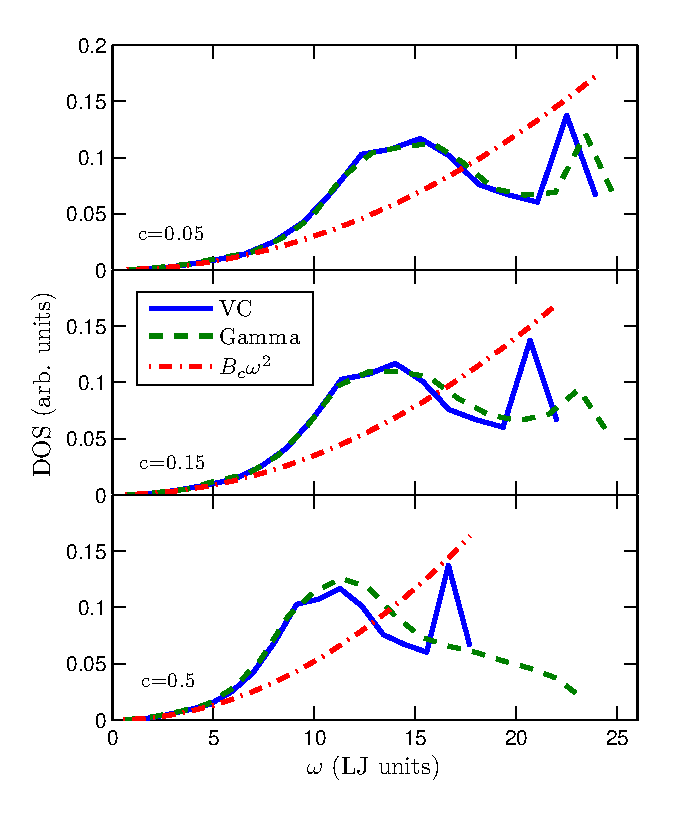
\includegraphics[scale=0.8]
{/home/jason/disorder/lj/alloy/lj_alloy_dos_c05-5_4.eps}
\vspace*{-5mm}
\end{center}
\caption{\label{F:DOS} Density of states (DOS) 
for modes calculated using the LJ FCC  
VC versus an explcitily mass disordered LJ FCC supercell 
(labeled Gamma) with varying mass concentration $c$ (Section ). 
VC and Gamma show similar low frequency behavior for all $c$. 
For increasing $c$, the frequencies of both VC 
and Gamma decrease, while the high frequency DOS for Gamma spreads and  
reaches up to a higher maximum frequency because of the explict disorder. 
The size of these supercells is $N_0 = 12$ (see Section ).
}
\end{figure}
%--------------------------------------------------------------------------

%--------------------------------------------------------------------------
\subsection{\label{S:Dispersion}Dispersion}
%--------------------------------------------------------------------------

%--------------------------------------------------------------------------
\subsubsection{\label{S:From VC}From VC}
%--------------------------------------------------------------------------

The group velocity vector in a VC is the gradient of the dispersion curves, 
\begin{equation}\label{EQ:Dynamical}
v_{g,\mathbf{n}}\kv = \partial \omega\kv / \partial \pmb{\kappa},
\end{equation}
 which can be 
calculated from the frequencies and wavevectors using finite differences. 
In this work, the group velocities for the VC are calculated 
using finite difference 
and quasi-harmonic lattice dynamics.\cite{mcgaughey_phonon_2006} 

In general, real systems have dispersion which depends on the wavevector 
and polarization.   
For simple systems, such as LJ argon, the 
dispersion has only 3 polarizations $\nu$, 
1 longitudinal and 2 transverse acoustic branches.
\cite{dove_introduction_1993} For SW silicon, the 2-atom basis creates 
optical modes which have distinctly different dispersions than 
acoustic branches, and hence have different group velocities.  For 
systems with a large basis or low-symmetry, 
the dispersion can be very complicated.(cite) 

Except for the three 
acoustic branches (2 transverse, 1 logitudinal), there is not an 
accepted method to predict the effective group velocity of a 
vibrational mode in a disordered system, though there are attempts.
\cite{cahill_lattice_1988,duda_reducing_2011,donadio_atomistic_2009,
he_heat_2011,he_thermal_2011} 
In the Cahill-Pohl (CP) model, the group velocity of all disordered 
modes is the sound speed $v_s$ (Section ).\cite{cahill_lattice_1988} 
Dispersion for a model disordered 1D system attributes  
the reduction of group velocities due to a 
zone-folding effect.\cite{duda_reducing_2011} 
In studies of disordered silicon systems, the group velocity of 
vibational modes was estimated using an interpolation scheme for 
small but finite wavevectors 
near [000]. 
\cite{donadio_atomistic_2009,he_heat_2011,he_thermal_2011} 
footnote
(We do not, in general, observe the required dispersion 
beavhior near the Gamma point to perform the interpolation 
for the LJ and SW systems studied in this work.
\cite{donadio_atomistic_2009,he_heat_2011,he_thermal_2011})

Feldman et al used the structure factor to predict an effective dispersion 
for a model of a-Si, but did not predict group velocities.
\cite{feldman_numerical_1999} 
Volz and Chen used the dynamic structure factor to predict the
dispersion of SW Si using MD simulation, which is a perfect system.
\cite{volz_molecular-dynamics_2000} As a method to predict mode group 
velocities, we examine the structure factor 
for the explictily disordered modes in the next section.

%--------------------------------------------------------------------------
\subsubsection{\label{S:From Structure Factor}
From Structure Factor of Gamma Modes}
%--------------------------------------------------------------------------

Calculating the structure factor of Gamma   
modes is a method to test for the plane-wave 
character of disordered modes at a particular wavevector and 
polarization. 
\cite{allen_diffusons_1999,feldman_numerical_1999} 
The structure factor is defined as\cite{allen_diffusons_1999} 
\begin{equation}\label{EQ:SLT}
S^{L,T}\kw = 
\sum_{\nu} E^{L,T}\kv
\delta (\omega-\omega\kv),
\end{equation}
where $E^{T}$ refers to transverse polarization and is defined as
\begin{equation}\label{EQ:EL}
E^L\kv = 
\left|
\sum_{l,b} 
\hat{\mathbf{\kappa}} \cdot e\kvba 
\EXP{i\pmb{\kappa}\cdot\mathbf{r}_0\ab{l}{b}} 
\right|^2
\end{equation}
and $E^{L}$ refers to logitudinal polarization and is defined as
\begin{equation}\label{EQ:ET}
E^T\kv = 
\left|
\sum_{l,b} 
\hat{\mathbf{\kappa}} \times e\kvba 
\EXP{i\pmb{\kappa}\cdot\mathbf{r}_0\ab{l}{b}} 
\right|^2.
\end{equation}
Here, $\mathbf{r}_0\ab{l}{b}$ refers to the lattice positions in the 
mass disordered atoms in the supercells, which are still spaitally ordered. 
Explicit disorder is accounted for in the mode frequencies $\omega\kv$ 
and eigenvectors $e\kvba$ which are calculated with 
$\mathbf{\kappa} = [000]$. 

Physically, $S^{L,T}\kw$ calculates 
the frequency spectrum required to create a wavepacket with 
well-defined wavevector and polarization.
\cite{allen_diffusons_1999,feldman_numerical_1999} The details of the 
calculation are given in Appendix. 
For a perfect lattice, the 
structrue factor peaks are delta functions centered at the phonon mode 
frequencies, indicating they are pure plane-waves. 
With increasing disorder ($c$), the structure factor spreads in width,  
particularly at high frequencies (Fig ) because the modes are no longer 
pure plane-waves. 
An effective dispersion can be extracted by locating the peaks in the 
structure factors, where the effects of polarization, virtual mass, and 
anisotropic dispersion can be observed (Fig. ). 
As the lattice VC mass becomes larger,  
the peaks in the structure factor shift to lower frequencies. 
The peaks in the structure factor are shifted to 
slightly 
higher frequencies than the VC predicted frequencies by 
up to only $\%5$. Similar good agreement can be seen with the disordered 
SW silicon lattices, while the structure factors are more complicated 
because of the optical modes. 
Because of this good agreement,  
we use the group velocities predicted by the VC dispersion for both
LJ argon and SW silicon 
with the VC-NMD and VC-ALD calculations for 
consistency and simplicity (Section and Appendix \ref{A:SF} ). We examine 
the validity of this choice of group velocity in Section . 
Well-defined peaks (see Appendix ) 
at all wavevectors are most likely due to the 
lattice structure of the disordered systems studied in this 
work. 
Typically, the structure factor for amorphous materials has well-defined 
peaks only for small wavevector, which is related to the thermal 
diffusivity of the disordered modes.
\cite{allen_diffusons_1999,feldman_numerical_1999}   

%--------------------------------------------------------------------------
\begin{figure}
\begin{center}
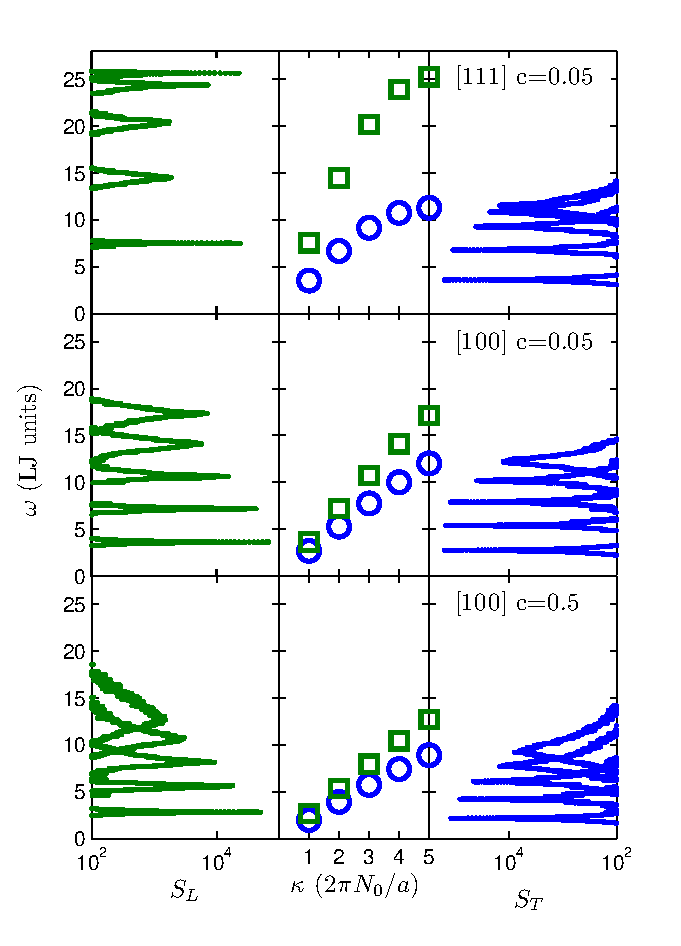
\includegraphics[scale=0.8]
{/home/jason/disorder/lj/alloy/lj_alloy_dsf_100_111.eps}
\vspace*{-5mm}
\end{center}
\caption{\label{F:SF} 
Left and Right Panels: 
The structure factor for logitudinal ($S_L$) 
and transverse ($S_T$) 
polarizations along high symmetry directions ([100], [110] 
where $\mathbf{\kappa}$ = $\pi/a[100]$ and $a$ is the 
lattice constant ) 
of the mass disordered LJ FCC supercells ($c=0.05,0.5$). 
For increasing 
mass disorder $c$, there is a decrease in the center of the peaks 
and an increase in the peak linewdiths. 
Center Panel:
The VC predicted dispersion at the same wavectors used to calculate 
$S_{L,T}$.
}
\end{figure}
%--------------------------------------------------------------------------

%--------------------------------------------------------------------------
\subsection{\label{S:Phonon Lifetimes}Lifetimes}
%--------------------------------------------------------------------------

%--------------------------------------------------------------------------
\subsubsection{\label{S:From VC Gamma}From VC-NMD and Gamma}
%--------------------------------------------------------------------------

As an alternative to the VC-ALD models for predicting phonon lifetimes 
(Section ), 
we use the normal mode decomposition (NMD) method.
\cite{ladd_lattice_1986,turney_predicting_2009} 
NMD maps the 
atomic trajectories (positions and velocities) of atoms in an MD 
simulation onto the vibrational normal mode coordinates,(cite)
\begin{equation}\label{E:q_HLD}
\begin{split}
q\kvt=&\SUM{0}{}\sqrt{\frac{m_b}{N}}u_{\alpha}\lbt e^*\kvba\EXP{i\pmb{\kappa}\cdot\mathbf{r}_0\ab{l}{0}}
\end{split}
\end{equation}
and
\begin{equation}\label{A:E:qdot_HLD}
\begin{split}
\dot{q}\kvt{}{}{}=&\SUM{0}{}\sqrt{\frac{m_b}{N}}\dot{u}_{\alpha}\lbt e^*\kvba\EXP{i\pmb{\kappa}\cdot\mathbf{r}_0\ab{l}{0}}.
\end{split}
\end{equation}
where $\mathbf{r}_0\ab{l}{0}$ are the equilibrium positions of the atoms 
in the $l$th unit cell of the lattice supercell under the VC approximation.
(needs work) 
The total energy of a given mode is given by 
\begin{equation}\label{A:E:qdot_HLD}
\begin{split}
E\kvt = \frac{\omega\kv}{2} q\kvt^*q\kvt + 
\frac{1}{2}\dot{q\kvt}^*\dot{q\kvt}
\end{split}
\end{equation}

The MD simulation is 
performed using the perfect and disordered supercells 
(Section, Fig. ). 
The NMD is performed using the frequencies and eigenvectors 
from both the VC ($\omega\kv$, $e\kvba$) and the Gamma supercell 
($\omega\kv$, $e\kvba$ with $\mathbf{\kappa}=[000]$, Section ). 
The vibrational mode frequencies and eigenvectors are necessary 
for the mapping of the atomic trajectories from the MD simulation 
onto the vibrational normal mode coordinates, 
$q\kvt and \dot{q}\kvt$, which are required 
to calculate the kinetic, potential, and total ($E\kv(t)$)  
vibrational normal mode energies.(cite) 
The effects of disorder enter through the trajectories from 
these MD simulations, which are also used for the GK method 
(Section ).

The normal mode lifetime is predicted using 
\begin{equation}\label{EQ:tau_nmd}
\tau\kv = \int_{0}^{\infty} \frac{<E\kvt E\kvzero>}{ <E\kvzero E\kvzero> }dt,
\end{equation}
where the indefinite integral is replaced by a finite integration given 
the specifications of the MD simulation. This method for predicting the 
mode lifetime is more robust than other methods for the disordered systems 
studied in this work (see Appendix \ref{A:NMD XCORR}). It does, however, 
make it more difficult to predict a phonon frequency, so we use the 
VC predicted frequency for all VC-NMD predictions, which allow for easier  
comparison to VC-ALD (Section ).

The lifetimes predicted using VC-NMD and Gamma-NMD  
are shown in Fig. First, the range of frequencies of the modes for 
VC-NMD and Gamma-NMD differ slightly, particularly at high frequency, 
which is due to the difference in the DOS (Fig. ). 
For small intervals of frequency, there are a wider range of 
predicted lifetimes for Gamma-NMD. This is because there is no symmetry 
averaging of the mode properties, which is performed for the modes 
of VC-NMD given that a VC is assumed.(cite)

Lifetimes predicted by both VC-NMD and Gamma-NMD show scalings with 
frequency which are predicted by the perturbative methods 
of VC-ALD (Section ), in 
particular scalings of $\omega^{-2}$, $\omega^{-4}$ and even faster 
scaling due to the DOS behavior (Fig. , Section ). What is not predicted by 
the perturbative VC-ALD methods is the behavior at the highest frequencies, 
where $\tau~constant$, which is seen roughly for both VC-NMD and Gamma-NMD, 
except at $c=0.5$ for VC-NMD. 
In general, the lifetimes predicted by both VC-NMD and Gamma-NMD  
are larger than the Ioffe-Regel (IR) limit,\cite{taraskin_determination_1999} 
\begin{equation}\label{EQ:IR}
\tau = 2\pi/\omega.
\end{equation}
The physical interpretation of the IR limit is that of a mode which 
scatters in a time less than its oscillation period, which is satisfied 
for most modes in Fig. At the highest frequencies, the existence of this 
characteristic (thought not exactly minimum) lifetime for LJ argon 
is analagous to the minimum mean free path used in a simple models 
of glasses.\cite{graebner_phonon_1986} There is, however, no theoretical 
prediction of this high-frequency behavior. 

While it is possible to predict a MFP given the VC predicted group 
velocities and the lifetimes predicted by VC-NMD, we find that it is not 
useful to understanding this high-frequency beavhior. For the group velocities 
predicted from the VC dispersion, they generally trend towards 
0 as the wavevector is increased to the BZ boundaries. This would predict 
a MFP of 0, which is not helpful to the current discussion. 
Furthermore, the concept of a MFP becomes poorly defined the more the system 
is disordered (e.g. dilute alloys to high concentration and amorphous phases). 
It is thus more useful to consider the proposed lower-limit of the  
mode thermal diffusivities, which combine the mode lifetime 
and effective group velocity, or equivalenty, effective MFP (Section ).

%--------------------------------------------------------------------------
\begin{figure}
\begin{center}
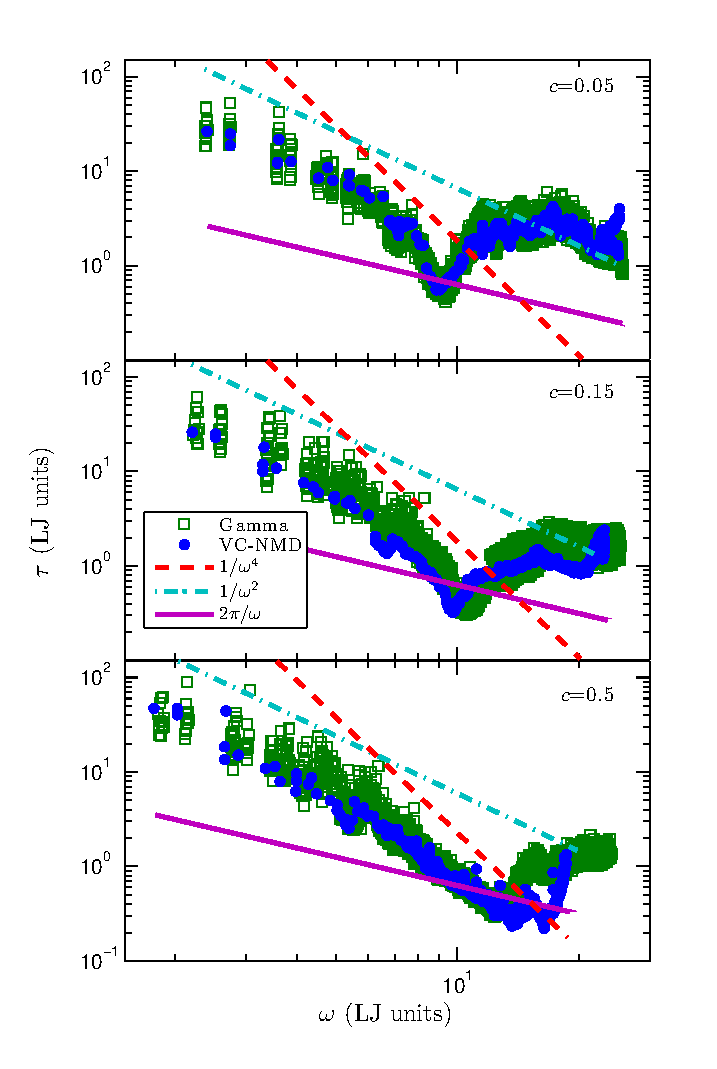
\includegraphics[scale=0.75]
{/home/jason/disorder/lj/alloy/lj_alloy_nmd_vc_gamma_life-2.eps}
\vspace*{-5mm}
\end{center}
\caption{\label{F:VC Gamma life} Lifetimes predicted using VC-NMD 
and Gamma NMD from MD simulations of mass disordered lattice supercells 
(Section ). Both $\omega^{-2}$ and $\omega^{-4}$ scalings can be observed 
at low frequencies, which are predicted by the peturbative models used 
for VC-ALD (Section ). For both VC-NMD and Gamma NMD, most mode 
lifetimes are greater than the Ioffe-Regel limit $\tau = 2\pi/\omega$. 
\cite{taraskin_determination_1999}
While there is more ``noise'' in the Gamma mode data (Section ), 
the lifetime magnitudes and 
trends agree well, an important consideration when comparing VC-NMD and 
VC-ALD in Fig. .
}
\end{figure}
%--------------------------------------------------------------------------


%--------------------------------------------------------------------------
\subsubsection{\label{S:From VC-ALD}From VC-ALD}
%--------------------------------------------------------------------------

Assuming initrinsic and disorder scattering mechanisms 
to operate independently, the 
effective phonon lifetime can be found using Matthiessen's rule(cite),
\begin{equation}\label{EQ:Matthiessen}
\frac{1}{\tau\kv} = \frac{1}{\tau_{p-p}\kv} + \frac{1}{\tau_{d}\kv},
\end{equation}
where $\tau_{p-p}\kv$ accounts for intrinsic phonon-phonon scattering 
and $\tau_{d}\kv$ accounts for defect scattering.

Phonon-phonon scattering ($\tau_{p-p}\kv$) is typically treated 
using anharmonic perturbation theory (ALD) including only 3-phonon 
processes.\cite{turney_predicting_2009,garg_role_2011,tian_phonon_2012} 
It has been demonstrated that the effects of higher order n-phonon 
processes become important at high temperatures (see Section ).
\cite{ecsedy_thermal_1977,turney_predicting_2009} 
At low frequencies where the density of states is Debye-like 
(Section Fig. ), 
$\tau_{p-p}\kv$ follows a scaling due to both normal ($B_1\omega^{-2}$) 
and umklapp ($B_2\omega^{-2}$) 3-phonon scattering processes, where the 
constants $B_1$ and $B_2$ are typically fit to experimental data.(cite) 
The scaling $\tau ~ \omega^{-2}$ can be observed  
in both the NMD (Fig. ) and ALD (Fig. ) predicted results. 

Using harmonic perturbation theory, Tamura gives a general expression 
for mass point defect scattering\cite{tamura_isotope_1983}
\begin{equation}\label{EQ:tau_d}
\begin{split}
\frac{1}{\tau_{d}\kv} = \frac{\pi}{2N}\omega^2\kv 
\sum_{\mathbf{\kappa'}\nu'} \delta( \omega\kv - 
\omega\kvp ) \\
\sum_{b} g_2(b) 
|e^*\kvbap \cdot e\kvba |^2 ,
\end{split}
\end{equation}
where 
\begin{equation}\label{EQ:g(b)}
\begin{split}
g_n(b) = \sum_\mu c^{\mu}(b)(1-m^{\mu}(b)/\bar{m}(b))^n, 
\end{split}
\end{equation}
N is the number of unit cells, and $c^\mu$ is the concentration, 
$m^\mu(b)$ is the mass of the $\mu$-th species 
and $\bar{m}^{\mu}$ is the average mass. 
For the binary LJ argon and SW silicon alloys considered, 
there is one atom type in the unit cell  
with $\mu=a,b$, so that the alloying atom labeled by $m^b_{1-c}$ 
can be considered to be an ``isotope'' of atom labeled 
$m^a_{c}$.  This convention is appropriate because of the 
perturbative approach used to derive Eq. , while we consider 
large disorder up to $c=0.5$.\cite{tamura_isotope_1983} 

The term $g_2(b)$ is a 
coupling term which defines the strength of the disorder which 
depends on the concentration and masses of the different species. 
(Give values of g for LJ and SW, at all $c=$ they are approimxately 
the same given the similar mass ratios used, so that the underprediction 
of VC-ALD for LJ argon is because of the nature of the system.)

needs work above

Bond disorder 
can be accounted for using a similar expression with an average
atomic radius or suitable scattering cross-section.
\cite{klemens_scattering_1955,klemens_thermal_1957} 
The effect of bond and mass disorder has been investigated computationally 
by Skye and 
Schelling for Si/Ge \cite{skye_thermal_2008}, 
where it was shown that mass disorder is 
the dominant scattering mechanism. In this work we consider only 
mass disorder.

By considering the symmetry properties of the FCC lattices 
considered in this work (Section ), it can be shown that
\begin{equation}\label{EQ:taud_dos}
\begin{split}
1/\tau_{d}\kv =\frac{\pi}{2} g_2 \omega^2\kv D(\omega\kv), 
\end{split}
\end{equation}
where 
$D(\omega\kv)$ is the density of states (Section ).
\cite{tamura_isotope_1983} 
Under the Debye-approximation ($D(\omega\kv)~\omega\kv^{2}$), 
the phonon scattering due to mass point-defects 
is given by $A\omega^{-4}$, where $A$ is a constant related to the unit 
cell volume, branch-averaged group velocity, and disorder coupling strength 
($g_2(b)$ in Eq. above). 
The frequency dependence ($\omega^4$) is the same as 
Rayleigh scattering, which is valid at low frequency and observed 
in both the NMD (Fig. ) and ALD (Fig. ) predicted results. 
The disorder 
scattering scaling is expected to fall off faster than $\omega^{-4}$ 
when $D(\omega\kv)$ grows faster than the Debye scaling of 
$\omega^{2}$ (Fig. , Section ). 
The lifetimes do fall off faster $\omega^{-4}$ for the 
mass disordered LJ FCC supercells for a narrow range of 
frequencies near $\omega = 10$ in Fig. for $c=0.05,0.15$, 
but seem to follow more closely $\omega^{-4}$ for $c=0.5$. 

For the VC-ALD method, 
the intrinsic $\tau\kv_{p-p}$ is calculated using the method described in
\cite{turney_predicting_2009}, using all classical expressions to remain 
consistent with the classical MD-based methods NMD and GK (Section ). 
To calculate the disordered lifetimes $\tau\kv_{d}$ (Eq. ), 
it is necessary to broaden 
the $\delta$ function using a Lorentzian function.[1] 
footnote[1]
For all calculations, the Lorentzian was broadened using a value of 
$100\delta_{\omega,avg}$ (Section ). For the system sizes here, 
the results do not differ significantly 
if this broadening value is varied manually or  
by increasing system size ($N_0$).

Higher-order terms in the Tamura theory can be represented by 
terms involving $g_n$ (where $b=1$, Eq. (Eq)) and $I(\omega)$, 
defined as 
\begin{equation}\label{EQ:taud_dos}
\begin{split}
I(\omega) = 
	    \frac{1}{6N}\sum_{\kv}
	    \frac{\omega\kv^2}{\omega\kv^2 - \omega - i\epsilon} , 
\end{split}
\end{equation}
where $\epsilon$ is a small number, taken to be 
$100\delta_{\omega,avg}$.  For example, the predicted frequency 
shifts due to disorder scattering are
\begin{equation}\label{EQ:taud_dos}
\begin{split}
\delta\omega/\omega = g_2(b) Re[I(\omega)]/2 , 
\end{split}
\end{equation}
and the terms $g_n|I(\omega)|^{n-2}/g_{n-1}$ represent estimates for the 
higher-order terms of the defect-perturbed phonon self-enegy (linewidth),
which are shown in Fig (Fig).\cite{tamura_isotope_1983} 
In the original study of isotope scattering 
in Ge, the perturbation was small and the higher-order terms were shown 
to be negligible. In the present study, which includes large 
amounts of disorder ($e.g.$ large values of $g_n$), the predicted 
frequency shifts and higher-order estimates are not small, especially 
at high frequency. The effect of these higher-order terms is important 
to understanding the results predicted by VC-ALD in Section and Section .

%--------------------------------------------------------------------------
\begin{figure}
\begin{center}
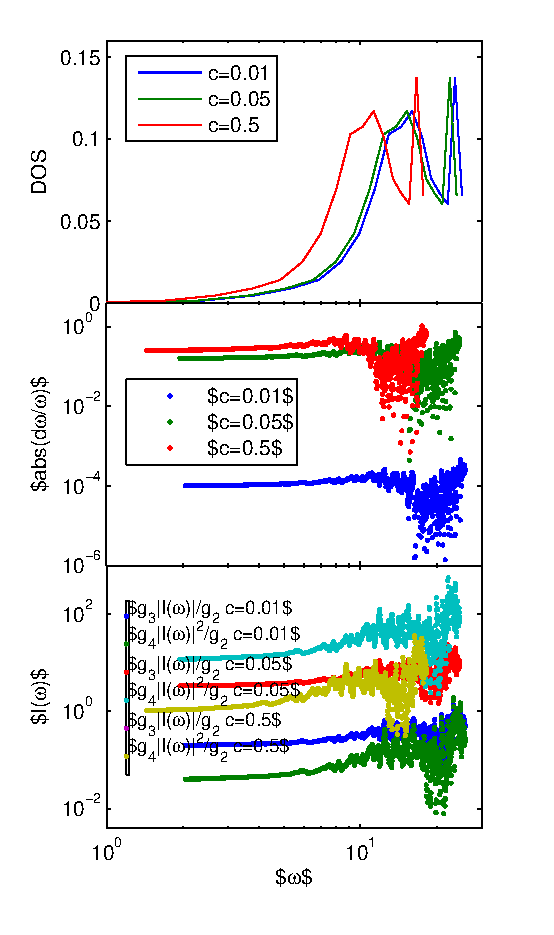
\includegraphics[scale=0.75]
{/home/jason/disorder/lj/alloy/m_alloy_tamura_highorder_compare_lj.eps}
\vspace*{-5mm}
\end{center}
\caption{\label{F:tamura_lj} lj tamura results}
\end{figure}
%--------------------------------------------------------------------------

%--------------------------------------------------------------------------
\begin{figure}
\begin{center}
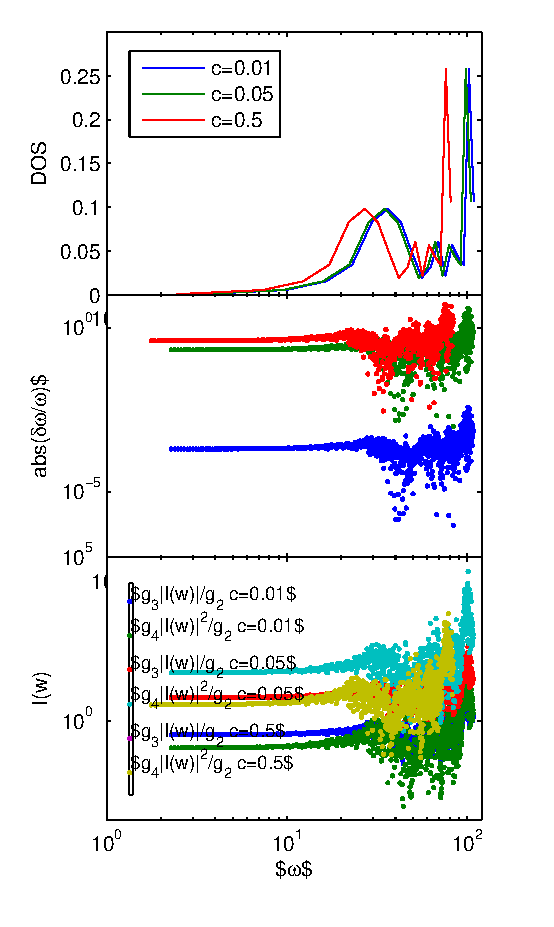
\includegraphics[scale=0.75]
{/home/jason/disorder/lj/alloy/m_alloy_tamura_highorder_compare_si.eps}
\vspace*{-5mm}
\end{center}
\caption{\label{F:tamura_sw} sw tamura results}
\end{figure}
%--------------------------------------------------------------------------

%--------------------------------------------------------------------------
\subsection{\label{S:Diffusivities}
Diffusivities}
%--------------------------------------------------------------------------

In the classical harmonic limit, where the specific heat $c_p\kv = k_{B}$, 
a vibrational mode's contribution to thermal 
conductivity is determined by the mode thermal diffusivity. For 
phonons, the thermal diffusivity is 
\begin{equation}\label{EQ:Dph}
D_{ph}\kv = \pmb{v}^{2}_{g}\kv \tau\kv.
\end{equation}
Here, $\pmb{v}^{2}_{g}\kv$ is calculated from the VC dispersion 
(Section ) for both VC-NMD and VC-ALD, so any differences in 
thermal diffusivity comes from the difference in the lifetimes 
predicted by these two methods. 

In explicitly disordered systems,  
modes can transport heat by harmonic coupling due to disorder 
in the Allen-Feldman (AF) theory of diffusons.\cite{allen_thermal_1993} The 
AF theory predicts the mode-specific thermal diffusivity of disordered 
vibrations. In the AF theory, the mode diffusivities typically diverges 
as $\omega -> 0$ because
the vibrational modes are long-wavelength plane waves (phonons) 
that weakly scattered by the disorder.
\cite{sheng_introduction_2006,vitelli_heat_2010}
footnote[]
(For the disordered lattices studied 
in this work for $c\le0.15$, the predicted $k_{AF}$ is strongly 
system size dependent, indicating this diverging behavior. 
For $c=0.5$, the divergence with system size is 
small for the range of system size studied ($N_0=4$ to $N_0=12$), 
where $k_{AF}/k_{GK} = 0.93$ for $N_0=12$.)

In the high-scatter (HS) limit,(cite) the AF diffusivity of each mode is
\begin{equation}\label{EQ:M:k_HS}
D_{AF,HS} = \frac{1}{3} v_s a,
\end{equation}
and the AF thermal conductivity prediction in the HS limit is
\begin{equation}\label{EQ:M:k_HS}
k_{AF,HS} = \frac{k_{B}}{V_b}b v_s a,
\end{equation}
where $V_b$ is the volume of the unit cell, $v_s$ is the 
branch-averaged sound speed, and $a$ is the lattice constant 
(or appropriate length scale,
although the choice of this length scale is not unique.).\cite{cahill_lattice_1988} 
A similar HS limit for mode diffusivity 
is given by the Cahill-Pohl (CP) HS model,(cite) $D_{CP,HS} = 0.403 v_s a$, which 
differs from the AF,HS model by a factor of approximately $\%20$.\cite{cahill_lattice_1988} 
Ignoring the small difference between the AF,HS and CP,HS models, 
the physical interpretation is of all vibrational 
modes with a group velocity equal to the sound speed 
and mean-free path equal to the 
lattice spacing. 
While the CP,HS and AF,HS models assume a constant thermal diffusivity for 
all modes, the AF theory is capable of predicting the mode specific 
diffusivities without any assumptions other than a harmonic 
approximation.(cite) 

With sufficient disorder, such as amorphous phases, the 
harmonic AF theory is capable of accurately predicting a finite 
thermal conductivity.
\cite{feldman_thermal_1993,shenogin_predicting_2009}  
The thermal conductivity of the LJ amorphous phase (with an effective 
mass of 2) is predicted by the AF theory, $k_{AF} = 0.099 W/m=K$.
footnote[]
(The amorphous LJ phase was created by liquifying the crystal 
and instantly quenching by removing all kinetic energy.  The resulting 
structure was then energy minimized and annealed in an NPT ensemble at 
zero pressure and $T=10$ K.(cite lammps))
The mode-specific thermal diffusivities for the LJ argon amorphous phase 
are shown in Fig. , where modes with significant 
contribution to thermal transport can be modeled using a mode-independent 
diffusivity of approximately $D_{AF,HS}$ (Eq. ). 
Also shown are the AF predicted thermal 
diffusivities for the explicitly disordered superlattice and $c=0.5$. 

While the AF theory is divergent in the low-frequency limit for lattices,  
the finite system size bounds the thermal diffusivities of the lowest 
frequencies (Fig ), and the thermal conductivity predicted by the AF theory 
is actually quite close to that predicted by the GK method, 
$k_{AF}/k_{GK} = 0.93$. More importantly, the thermal diffusivity of all 
modes in the explicitly disordered lattice supercell are finite, except 
at the highest frequencies where they tend to 0 as in the amorphous 
phase (Fig ). 
This places a plausible lower-bound on the value of the VC phonon mode 
diffusivities, $D_{ph} \ge D_{AF,HS}$. In fact,
the thermal properties of disordered lattices and glasses
has been explained heuristically by assuming that phonons
are scattered so strongly by structural disorder that transport 
becomes diffusive, with a frequency regime of small,
constant thermal diffusivity.
\cite{kittel_interpretation_1949,sheng_heat_1991}

The lower-limit of the thermal diffusivity predicted for the VC 
modes is $D_{ph}\kv \approx 0$, as is the case for the VC mode 
MFP because of the VC predicted group velocities (Section ). In typical  
explicitly disordered system, this lower limit of the thermal diffusivity 
is only seen for a minority of modes at the highest frequencies, which 
is true for the disordered LJ systems shown in Fig. 
Feldman et al showed that the thermal 
diffusivities in a-Si show a sharp breakpoint at the on-
set of localized states, where it tends to zero exponentially. 
Similar behavior is seen for the LJ argon disordered superlattices 
and amorphous phase 
($c=0.5$, Fig. ). 
%where it can be shown that these states are 
%spatially Anderson-localized by examining the eigenvector.(cite)

For both VC-NMD and VC-ALD, a significant number of modes have 
$D_{ph} \lt D_{AF,HS}$ (Fig. ). This can lead to an underprediction of the 
total thermal conducitvity. The diffusivity of these 
modes can be adjusted such that any mode with $D_{ph} \lt D_{AF,HS}$ is 
given $D_{ph} = D_{AF,HS}$.  The result of this adjustment, referred to as 
VC-NMD* and VC-ALD*, is examined 
in the thermal conductivity predictions in Section.

For LJ argon, VC-NMD predicts lifetimes which 
are generally larger than the period 
($\tau\kv > 2\pi/\omega\kv$)
of the vibrational oscillation (Ioffe-Regel limit)(cite), 
and actually increase then remain approximately constant 
at high frequency (Section and Fig. ).  
VC-ALD predicts essentially monotonically 
decreasing lifetimes with increasing frequency for both LJ argon and SW 
silicon (Fig. ). Because VC-NMD and VC-ALD 
use the same values for $v_g\kv$, the phonon mode 
diffusivities $D_{ph}\kv$ are also underpredicted for 
VC-ALD compared to VC-NMD. There are thus 2 underpredictions to consider 
when predicting the thermal conductivities in Section : underprediction 
of the thermal diffusivity assuming the VC phonon modes for 
VC-NMD and VC-ALD, and the underprediction of the mode lifetimes by 
the VC-ALD perturbative models. 

not used, yet...

energy transport in jammed sphere packings\cite{xu_energy_2009}
heat transport in model jammed solids\cite{vitelli_heat_2010}

%--------------------------------------------------------------------------
\begin{figure}
\begin{center}
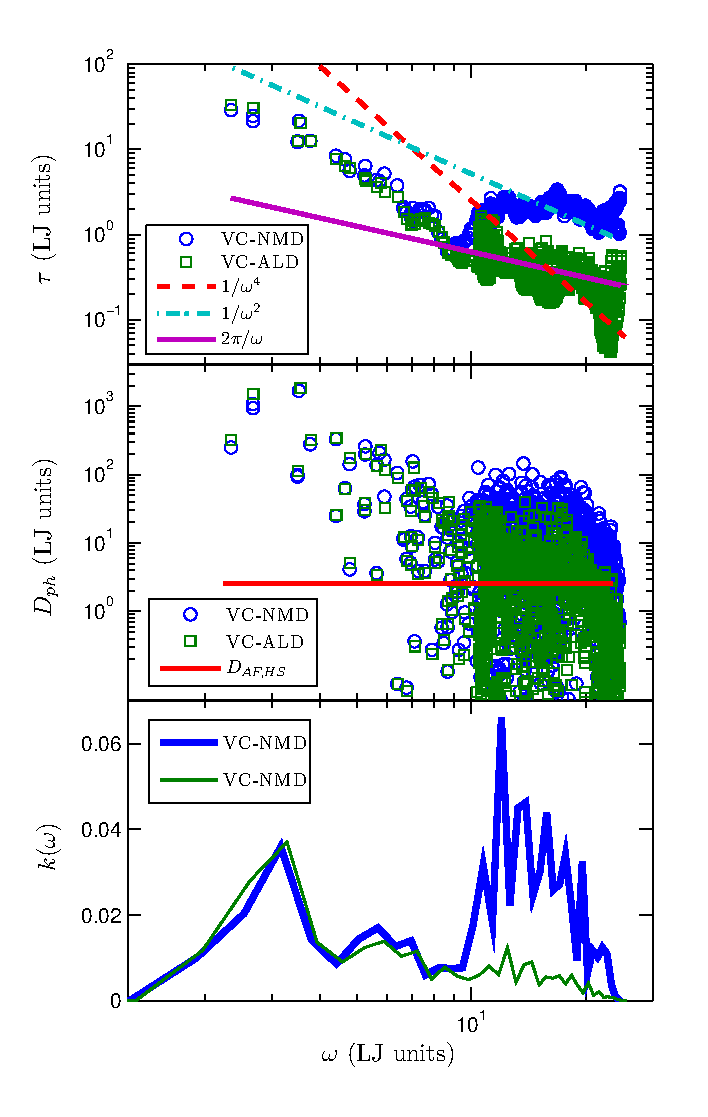
\includegraphics[scale=0.75]
{/home/jason/disorder/lj/alloy/af_nmd_ald_tau_diff_kw_c05_3-2.eps}
\vspace*{-5mm}
\end{center}
\caption{\label{F:Dph_lj} (a) predicted lifetimes for VC modes using 
VC-NMD and VC-AlD for LJ argon. 
(b) predicted VC mode thermal diffusivities, compared  
to the AF,HS limit. (c) the thermal conducitivty frequency spectrum, 
which is peaked at high frequency, in contrast to SW silicon (Fig).}
\end{figure}
%--------------------------------------------------------------------------

%--------------------------------------------------------------------------
\begin{figure}
\begin{center}
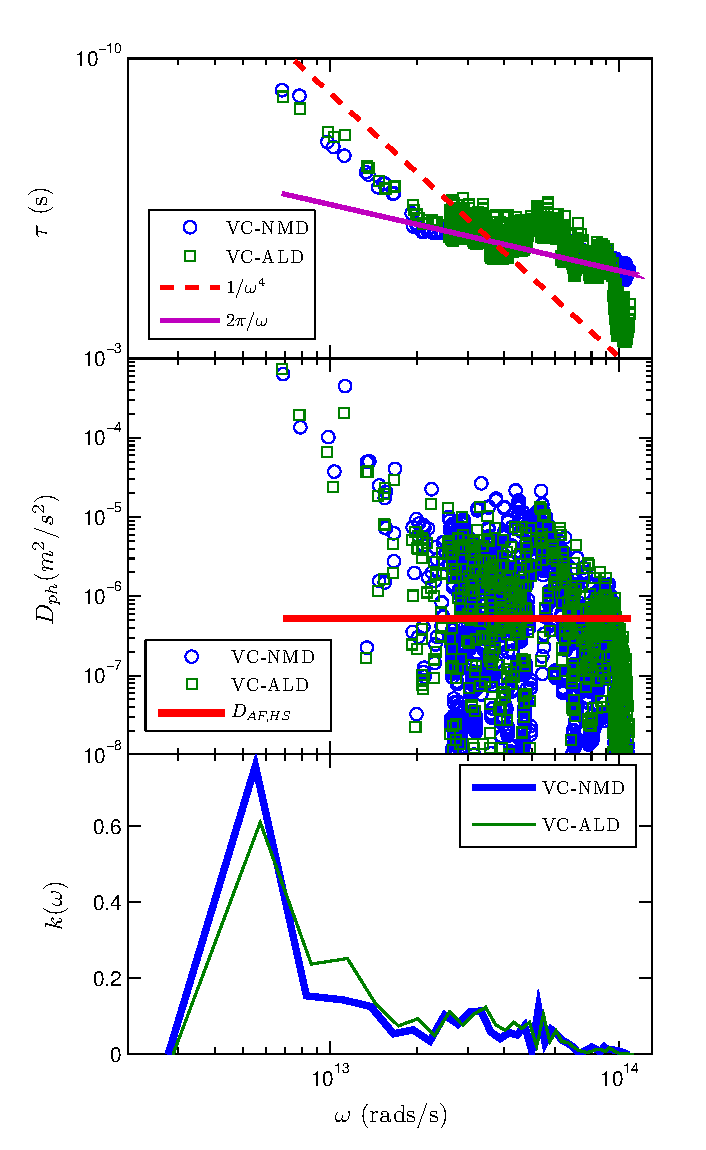
\includegraphics[scale=0.75]
{/home/jason/disorder/si/alloy/af_nmd_ald_tau_diff_kw_c05_2-2.eps}
\vspace*{-5mm}
\end{center}
\caption{\label{F:Dph_si} (a) predicted lifetimes for VC modes using 
VC-NMD and VC-AlD for SW silicon. 
(b) predicted VC mode thermal diffusivities, compared  
to the AF,HS limit. (c) the thermal conducitivty frequency spectrum, 
which is peaked at low frequency, in contrast to LJ argon (Fig). }
\end{figure}
%--------------------------------------------------------------------------

%--------------------------------------------------------------------------
\begin{figure}
\begin{center}
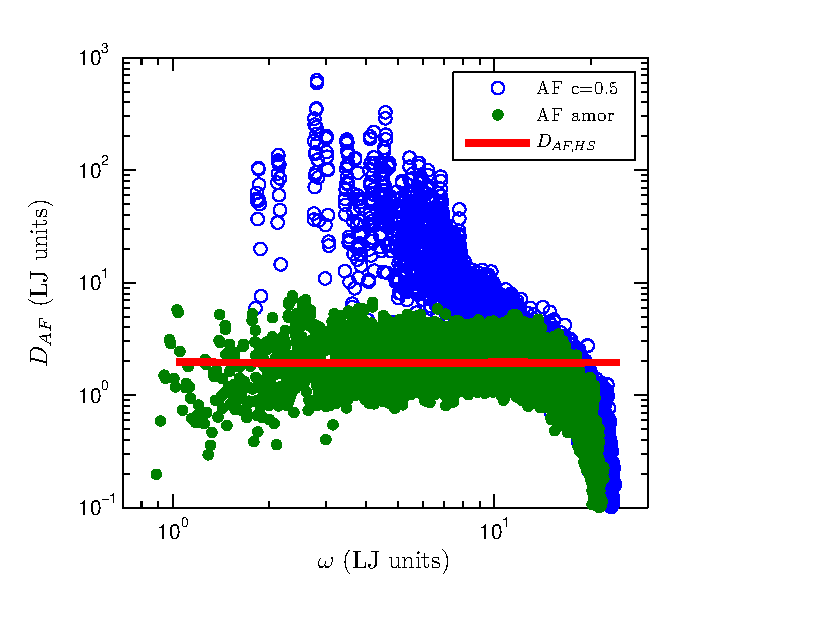
\includegraphics[scale=0.75]
{/home/jason/disorder/lj/alloy/af_c5_amor_DAF_kw_2.eps}
\vspace*{-5mm}
\end{center}
\caption{\label{F:AF} AF theory predictions of disorded mode  
thermal diffusivities for LJ argon disorded lattice supercell and 
amorphous phase. The mode thermal diffusivities predicted for the 
disorded lattice supercell are all finite, except at the highest 
frequency where they tend to 0 as in the amorphous phase. }
\end{figure}
%--------------------------------------------------------------------------


%--------------------------------------------------------------------------
\section{\label{S:Thermal Conductivity}Thermal Conductivity Predictions}
%--------------------------------------------------------------------------

The thermal conductivity can be predicted using the mode properties 
predicted by the VC-NMD and VC-ALD 
methods.  However, given the discussion of the mode properties 
preceeding this section, it is necessary to implement a third method 
for predicting thermal condudctivity. 
We choose the equilibirum MD-based green-kubo (GK) method.  This method 
does not predict any mode-specific properties, and is thus a system-level 
prediction.  For this reason, thermal conductivity predicted by GK 
has been shown to capture the effects of whatever scattering meachanisms are 
present in the MD simulation without any other assumptions (other than 
those which come with the classical nature of the MD siulation).(cite) 
Details of the GK and MD simulations are given in Appendix. 

For LJ argon, bulk thermal conductivity predictions are made for 
VC-NMD, VC-ALD and GK (Fig. ). For SW silicon, bulk thermal conductivity 
predictions can only be made for VC-ALD and GK because of the 
limited system size used for VC-NMD (see Appendix ). 
For LJ argon, both VC-NMD and VC-ALD underpredict the thermal 
conductivity compared to GK. 

From Fig. it is clear that both VC-NMD and VC-ALD underpredcit compared 
to GK.  The underprediction is only modest for VC-NMD, on the order of 
$20\%$ or less for all $c$. By adjusting the mode diffusivity as suggested 
in Section , the thermal conductivtiy predicted by VC-NMD$^*$ is brought 
into agreement with GK by approximately $10\%$ or less for all $c$. When 
combined with the high-scatter limit, this suggests that the mode properties 
predicted by VC-NMD are a fair representation of the explicitly disorderd 
modes used in the MD simulation.

The VC-ALD method underpredicts the thermal conductivity for all $c$, where 
the underprediction is worst at $c=0.5$ where $k_{VC-ALD} / k_{GK} = 0.56$ 
and is well outside the error bars of the calculations (which are on the order 
of the large symbol sizes in Fig. ). By applying the high-scatter limit 
adjustment VC-ALD$^*$, the thermal conductivities are brought into marginally 
better agreement, worst for $c=0.05$ where $k_{VC-ALD^*} / k_{GK} = 0.65$. 
This is because of the underprediction of the mode lifetimes at high frequency 
for VC-ALD compared to VC-NMD in Section , since the two methods share the 
same mode group velocities. 

The failure of the VC-ALD method can be demonstrated further 
by moving to higher temerpature ($T=40$ K Fig. ).
The beginning breakdown of the intrinsic scattering model 
($\tau_{p-p}\kw$) can be observed for the perfect ($c=0.0$) crystal at 
$T=40$ K (see Fig. ), where ALD begins to overpredict compared to GK.  This 
can be explained by the emerging importance of higher order (n$> 3$) 
n-phonon process at high temperatures.\cite{turney_predicting_2009} 
While the VC-ALD method begins to overpredict at this elevated temperature, 
it continues to underpredict for the alloys $c \ge 0.05$.  In fact, the 
thermal conductivity predicted by VC-ALD is right at (and slightly below) 
the HS limit. This demonstrates that the VC-ALD method is failing to 
accurately predict the high frequency mode lifetimes similar 
to $T=10$ K. The thermal diffusivity adjusted VC-ALD$^*$, again, is 
only marginally improved. 

Because the mode lifetimes are underpredicted at high frequencies for 
VC-ALD compared to VC-NMD, this leads to an underprediction for VC-ALD 
of both the thermal conductivity spectrum (Fig. ) at high 
frequency and the total thermal conductivity (Fig. ) 
compared to VC-NMD and GK (Section ). 
As noted in Section , for LJ argon in the amorphous phase, 
$k_{GK} = $0.121 W/m-K and $k_{CP,HS} =$ 0.12 W/m-K, indicating that 
almost all important modes to thermal transport are high-scattering. The GK 
predicted thermal conductivity predictions for the disordered lattices 
demonstrate that there are 
important contributions from propagating modes, even at higher temperatures 
where $k_{GK} > k_{AF,HS}$. 

For SW silicon, the thermal conductivities prediction by VC-ALD and GK 
are in good agreement, even without the adjustment VC-ALD$^*$, which only 
increases the result from VC-ALD by about 1$\%$. 
In SW silicon, even the amorphous phase has significant contributions 
from propagating modes which are considered to be phonons.(cite) Without 
any detailed mode-by-mode analysis, comparing the thermal 
conductivity predicted for the 
SW silicon amorphous phase ($k_{GK} \approx$ 3 W/m-K (cite)) compared to 
the HS limit, 
$k_{AF,HS} = $0.5 W/m-K, demonstrates that there is significant 
contribution from what can be considered propagating modes.(cite)  
In fact, for a-Si, the mode diffusivities vary as a function 
of frequency,
\cite{feldman_thermal_1993,feldman_numerical_1999,allen_diffusons_1999} 
which has been used to explain the propagating 
mode effects seen in a-Si thin films.\cite{he_heat_2011}



%--------------------------------------------------------------------------
\begin{figure}
\begin{center}
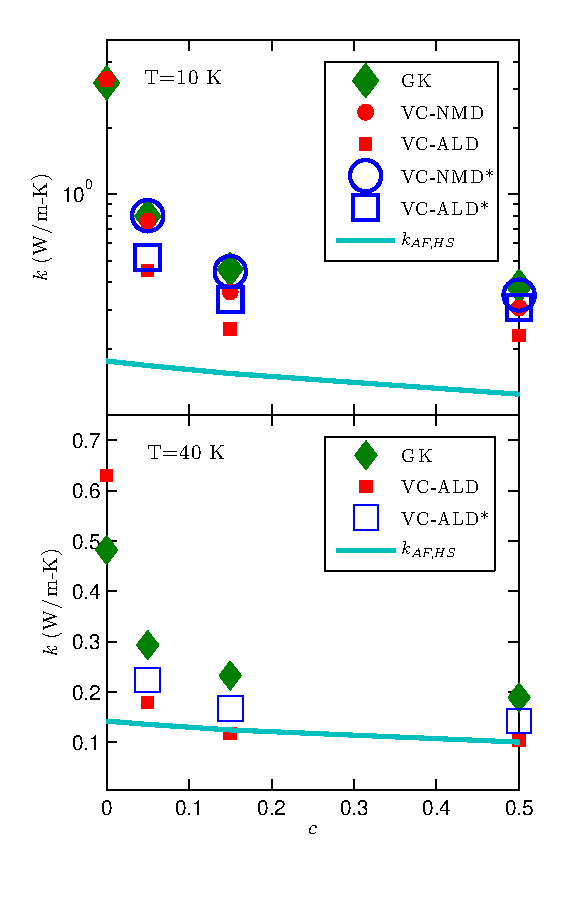
\includegraphics[scale=0.75]
{/home/jason/disorder/lj/alloy/lj_cond_compare.eps}
\vspace*{-5mm}
\end{center}
\caption{\label{F:conductivity_lj} }
\end{figure}
%--------------------------------------------------------------------------

%--------------------------------------------------------------------------
\begin{figure}
\begin{center}
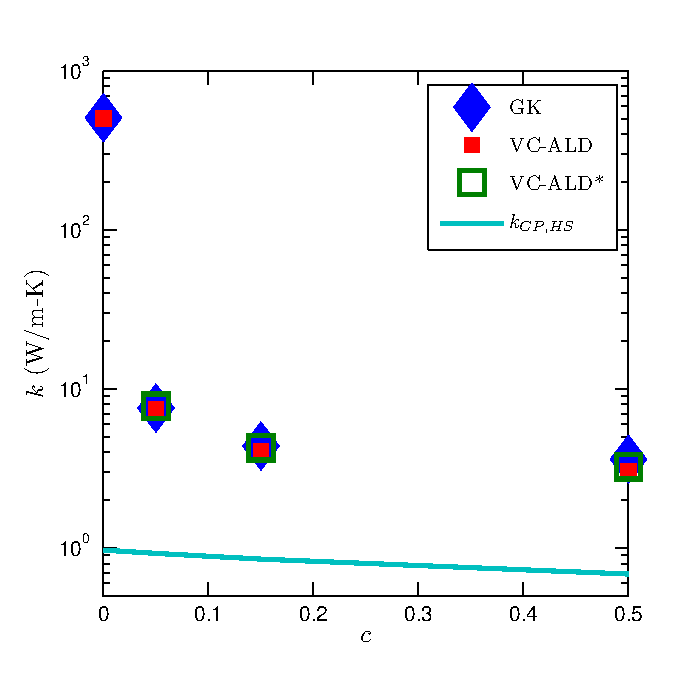
\includegraphics[scale=0.75]
{/home/jason/disorder/si/alloy/si_cond_compare.eps}
\vspace*{-5mm}
\end{center}
\caption{\label{F:conductivity_si} }
\end{figure}
%--------------------------------------------------------------------------


%--------------------------------------------------------------------------
\section{\label{S:Discussion}Discussion}
%--------------------------------------------------------------------------

By enforcing the lower-limit of 
thermal diffusivity, the thermal conducitvity of  . The importance of this 
result 

While the AF theory is divergent for lattices in the infinite-size limit, 
the theory provides a plausible lower-limit for a vibrational mode's 
thermal diffusivity, particularly at high frequencies 
where the mode lifetime and group velocity (or MFP) cannot be independently 
defined.\cite{feldman_numerical_1999,xu_energy_2009} 
This ambiguity can be resolved by 
considering the thermal diffusivity of a given mode, which incorporates 
the variation of both group velocity and lifetime (see Section ).

Based on the results locating the peaks in the structure factors 
(Fig. ), the reduction due to zone folding 
would seem to underpredict the group velocity of 
moderate to high frequency modes.\cite{duda_reducing_2011} Instead, 
the VC predicted group velocities, when coupled with the VC-NMD predicted 
mode lifetimes and thermal diffusivity adjusted VC-NMD$^*$, 
predict thermal conducitivities in good agreement with 
the MD-based GK method. 

There is a clear breakdown of the perturbative models used in  
VC-ALD (Fig. LJ-Diff and Fig. LJ thermal cond 40K), 
Because of its computational efficiency (Appendix ) a simple correction 
VC-ALD* is useful. This correction brings the predictions for LJ argon 
into better (though not great) agreement with the MD-based methods, and 
does not affect the good agreement seen in SW silicon (Fig. ). 

The existence of a minimum or characteristic mode lifetime for 
LJ argon (Fig. ) is suggested heuristically based on similar limits 
for electron transport.(cite) Such a minimum, defined in terms of the mode 
mean free path was, was proposed to explain the plateau 
temperature dependance of glasses.\cite{graebner_phonon_1986} 
There is difficulty in converting 
between lifetime and mean free path because of the inability to 
define an effective group velocity for all but the low frequency modes. 
In this work, the Ioffe-Regel limit ($\tau = 2\pi/\omega $) seems to be 
a lower limit for the mode lifetimes except for those predicted 
using VC-ALD (Fig. LJ-Gamma, LJ-Diff and SW-Diff ). 

For LJ argon, it is possible that the VC group velocities are an over-prediction 
for modes in a given interval of frequency, 
but is compensated for 
by an under-prediction of the lifetimes in the same interval of 
frequency when compared to the Gamma modes (Fig. ). The only constraint 
we have to compare against is the total vibrational conductivity, which 
shows good agreement for VC-NMD compared to GK. 

Use of the VC approximation is a theoretically and 
computationally simple way to predict a representative group velocity.

As observed by Kittel, if the sound
velocity is used instead of U; and the interatomic spacing
is used instead of the mean free path l;, then tc( T) is qual-
itatively and semiquantitatively
fit at temperatures above
the plateau region.
In fact, Slack showed that the same model 
is useful for crystalline insulators with strong scattering.(waiting for 
ILL).\cite{henry_ehrenreich_thermal_1979}

While there is no theoretical justification for 
the lower limit to the the mode mean-free path.\cite{graebner_phonon_1986} 
For the lattices studied in this work, the more appropriate quantity to 
consider is the mode diffusivity since both the 
effective mode lifetime   
and group velocity are varying with frequency (Fig. ). 
Since the Allen-Feldman theory does not rely on the assump-
tion of propagating phonons we expect the results for d͑␻͒
to be valid even in the high-frequency regime, where the
diffusivity cannot be factorized into a product of $l(\omega)$ times
a frequency-independent speed of sound.

In these ordered and disordered lattices, it is difficult to separate 
the contributions to the total vibrational 
conductivity from $D_{ph}\kv$ and $D_{AF}$ unless the lower limit 
$D_{CP,HS}$ or $D_{AF,HS}$ are used.  

The theory by Tamura is able to treat disorder scattering in an arbitrary 
crystal with dispersion. The theory, however, fails to predict the 
lifetimes of high-frequency modes, which are critical to the total 
thermal conductivity in LJ argon (see Fig. and ). To match the predicted 
phonon lifetime at high fequency for $c=0.05$ 
($\tau\kv \propto const.$, Fig. ), 
the Tamura theory (to order 2, $g_2(b)$) requires a DOS which scales as 
$D(\omega\kv) \propto const.$. Clearly from Fig. , this is not the case 
with either the VC or Gamma modes. To match the predicted 
phonon lifetime at high fequency for $c=0.5$ 
($\tau\kv \propto 1/\omega\kv$, Fig. , also true for all $c$ in SW silicon), 
The higher-order terms in the Tamura theory are demonstrated to be large 
in Fig., but it is unclear if and how they are responsible for the 
underpredictions of the VC-ALD method for LJ argon. 

While Broido found that omission of optical scattering overpredicts 
the thermal 
conductivity of bulk Si by a factor of 2-3, 
optical modes contribute less than $5\%$ 
to thermal conductivity itself. Similarly, the diffusivity adjusted thermal 
cobductivities of SW Si are increased by less then about $1\%$, demonstrating the 
the high frequency and optical modes are also unimportant to thermal transport 
in Si alloys. 

For the perfect system, phonon modes with nearly zero group velocity 
(optical modes and acoustic modes at the BZ boundaries) have essentially 
zero thermal diffusivity and contribute nearly 
nothing to the thermal transport, while the modes themselves 
are important to the 
scattering of other phonons.(cite) In the disordered lattices under the 
AF theory, modes important to thermal transport have a finite thermal 
diffusivity, as opposed to  the minimum $D_{th} \approx 0 $ for phonons 
in a perfect lattice. This finite thermal diffusivity limit is the cause 
for the large (LJ argon Fig. ) and small (SW silicon Fig. ) 
descrepcny between the thermal conductivity prdictions of VC-ALD and 
VC-NMD versus 

High thermal conductivity materials tend to have a conductivity spectrum 
which is peaked in the low frequency range.(cite) 
It is in this range where the mode 
lifetimes follow closely the scalings with frequency which can be 
predicted by the perturbative models for intrinsic and disorder scattering as 
(Section Eq. ).

In contrast, 
in LJ argon the high frequency phonon mode properties are critical 
to the thermal transport.(cite)  
While the low frequency phonon properties predicted by VC-NMD and 
VC-ALD agree, it is the failure of the perturbative models at 
high frequency which causes VC-ALD to underpredict. The failure 
to account for harmonic disordered scattering due to the AF theory 
is responsible for causing both VC-NMD and VC-ALD to underpredict 
versus GK, which affects the high frequency modes significantly. 
LJ argon, with lower 
frequencies, lifetimes, and group velocities compared to 
``stiff'' SW silicon, 
is considered a ``soft'' system. The predictions using 
VC-NMD, VC-ALD demonstrate the importance of explicit disorder 
modeling in ``soft'' systems and possible underprediction 
of the thermal properties.\cite{tian_phonon_2012}

For SW silicon, the low frequency modes dominate thermal transport 
even in the heavily disordered alloy.(cite new Hopkins) 
It is thus unsurprising that predictions for 
SW silicon using VC-ALD agree well with VC-NMD and GK. This is also a 
plausible explanation for the success of predictions using 
VC-ALD and ab initio calculations compared to experiment for 
``stiff'' systems (i.e. Si-Ge).(cite)

%--------------------------------------------------------------------------
\section{\label{S:}Summary}
%--------------------------------------------------------------------------

Results in this work suggest that the lower limit for the mode diffusivity 
lattices with thermal conductivities which are near the 
high-scatter limit.

\begin{acknowledgements}
This work was supported in part by a grant of computer time from the DOD 
High Performance Computing Modernization Program at the US Army Engineer 
Research and Development Center. 
We thank Jivtesh Garg, Zhiting Tian, Davide Donadio, 
Asad Hasan and Craig Maloney for helpful discussions.
\end{acknowledgements}

%--------------------------------------------------------------------------
\appendix
%--------------------------------------------------------------------------

%--------------------------------------------------------------------------
\section{\label{A:Computational Cost}
Computational Cost}
%--------------------------------------------------------------------------

The key to incorporating the effects of disorder explicitly are the use 
of a large disordered supercells (Section ).  However, the methods used 
in this work scale differently with the size of the supercell considered. 
The calculations in this work are trivially parallelizable\cite{} 
except the 
MD simulations\cite{plimpton_fast_1995} and the eigenvalue solution of the 
Dynamical matrix (Section ).\cite{gale_general_2003} Efficient MD 
codes scale linearly with the number of atoms in the system $N_a$, making 
the GK method an efficient method for predicting thermal conductivity. 
However, the computational cost of using large supercells for MD simulation, 
particularly because of the large number of time steps required 
(on the order of $10^5 - 10^7$ depending on the 
system, time step used, etc (cite)), prohibit its use with typical 
ab initio methods such as plane-wave Density Functional Theory.(cite) 

Both VC-NMD and VC-ALD require the eigenvalue solution 
of a Dynamical matrix of size $(3n,3n)$ for each irreducible wavevector 
of the system size considered (Section ), 
which is negligible compared to the other 
caculations required for both of these methods.(cite) 
The Gamma-NMD (Section ) and AF theory (Section ) 
require the eigenvalue solution of a large Dynamical matrix $(3N_a,3N_a)$, 
the solution of which scales as $(3N_a)^3$ (Section ). 
The AF theory is limited 
to small supercells using ab initio calculations, making it difficult 
to asses finite-size effects (Section ).  

Using the VC-ALD method, the symmetries of the system can be 
used to drastically reduce the required computations, permitting its 
use with ab initio methods.
\cite{esfarjani_method_2008,turney_predicting_2009,
esfarjani_heat_2011,chaput_phonon-phonon_2011} 
For VC-ALD, the calculation of the intrinsic phonon 
lifetimes $\tau_{p-p}\kv$ scales as $n^4$,\cite{turney_predicting_2009}  
making calcualtions for large unit cells challenging.(cite) 
Compared to 
the calculation of the intrinsic phonon lifetimes, calculation 
of the defect lifetimes $\tau_d\kv$ (Eq. ) is negligible.

% Consider the following computational times for the methods used in 
% this work for LJ argon and $N_0 = 12$. All calculations were performed 
% on the same computing cluster and include the effect of using 
% multiple processors (for example the VC-ALD calculations were run using 
% 12 cpu for 4.1 hours):
% 
% AF = eigenvalue solution + thermal diffusivity calculation = 4.2 hours
% 
% VC-ALD time = 49.2 hours?
% 
% VC-NMD time = 102 hours for MD + 780 hours for NMD + negligible time 
% to generate phonon frequencies and eigenvectors
% 
% LJ VC-Gamma = MD simulation + NMD + eigenvalue solution =  
% 102 hours + 780 hours + 3.8 hours = 
% 
% Parallel eigenvalue solvers exist for most ab initio packages, required 
% to solve for the eigenvalues of the Hamiltonian matrix.(cite) Incorporating 
% parallel eigenvalue solvers into existing 
% Sparse eigenvalue solutions may be implemented for systems which are 
% large enough and have short-range interactions.(cite)

% \begin{center}
% \begin{table}
% \caption{\label{T:cond_table}Thermal conductivity values in W/m-K predicted using the $\Phi$, 
% $\Phi'$, and Green-Kubo methods.  The predictions for $\Phi$ and Green-Kubo for the LJ system 
% are in good agreement with those from other atomistic simulation methods\cite{turney2009a} while 
% those from $\Phi'$ differ and show no consistent behavior. The uncertainties in the predicted thermal 
% conductivities for $\Phi$ and $\Phi'$ come predominantly from the finite simulation-size scaling 
% procedure (see Ref. \cite{turney2009a,He2011a}), where the phonon properties and thermal conductivity 
% are predicted for increasing system sizes ($N_1=N_2=N_3$) to extrapolate a bulk thermal conductivity. 
% For SW silicon and the CNT, the extrapolation procedure is not performed. }
% \begin{ruledtabular}
% \begin{tabular}{llllll}
%      &                             &         &      &   \\
% $T$ (K)&Green-Kubo \ &$\Phi$ &$\Phi'$\\
% \hline
% LJ (bulk)\\
% 5&8.0 $\pm$ 0.30 &7.9 $\pm$ 0.42 &5.8 $\pm$ 0.31 \\
% 20&1.3 $\pm$ 0.15 &1.2 $\pm$ 0.07 &1.0 $\pm$ 0.10 \\
% 40&0.45 $\pm$ 0.07 &0.47 $\pm$ 0.03 &0.49 $\pm$ 0.05 \\
% \hline
% SW ($N_1=N_2=N_3=6$) \\
% 300& &322 $\pm$ 16 &396 $\pm$ 38 \\
% \hline
% CNT ($N_1=N_2=1, N_3=50$) \\
% 300& &428 $\pm$ 21 &398 $\pm$ 40 \\
% \end{tabular}
% \end{ruledtabular}
% \end{table}
% \end{center}

%MD: Loop time of 2021.86 on 12 procs for 1000000 steps with 6912 atoms
%matlab NMD: /home/jason/lammps/LJ/alloy/10K/0.5/12x/NMD/1
%35261.719809 for one NMD_1_1

%--------------------------------------------------------------------------
\section{\label{A:NMD XCORR}
NMD using Non-Exact Normal Modes}
%--------------------------------------------------------------------------

The NMD method reuquires the atomic trajectories (positions and velocities) 
from an MD simulation. 
The MD simulations are performed using the package LAMMPS.
\cite{plimpton_fast_1995} The lengths of the MD simulations were longer 
than 10 times the longest phonon lifetime in the system. These can 
be estimated a priori from the VC-ALD predicted phonon lifetimes. For LJ 
argon and SW silicon, the simulations were run using time steps of 
$dt=0.002$ LJ units and $dt = 0.0005 fs$ for $2^20$ and 
$2^22$ time steps and the atomic trajectories were sampled 
every $2^8$ and $2^4$ time steps, respectively. 
Ensemble averaging was performed using 10 independent initial 
randomized velocity distributions. 

For a normal mode which is a normal mode of the lattice supercell 
used for the MD simulations (Section ), 
the autocorrelation of the total and kinetic     
normal mode energy are damped exponentials 
with a decay time $\tau\kv$, the kinetic energy autocorrelation with a 
cosinusodial oscillation frequency 
$2\omega\kv$.(cite joe) 
When using the VC normal modes (Section ) to map the MD simulation 
trajectories for the explicitly disordered lattice supercells (Section ), 
the mode total and kinetic energy autocorrelation fucntions 
do not always follow simple functional forms. 
This can be illustrated by using spectral-NMD 
in the frequency domain, where artifacts such as 
multiple peaks in an isolated mode's 
energy spectrum ($\Phi$) can be observed (see Fig ).(cite)  
In the case 
of multiple peaks, the choice of which peak to fit to predict the phonon 
properties can be ambiguous.  However, 
a lifetime can be predicted unambiguously using Eq. even with 
these multiple-peak artifacts, particularly because the autocorrelations 
are damped exponentially. This results is to be expected 
given that the atomic trajectories contain 
information about the lattice energy, which from general statistical 
physics principles will have exponential relaxation behavior in an 
equillibrium ensemble.
\cite{srivastava_physics_1990,landau_statistical_1980,
rajabpour_thermal_2010}

These artifacts are not surprising given two considerations: 
1) the MD simulations 
contain explicit disorder which incluences the atomic trajectories 2)
the VC normal modes are not the exact normal modes and of the 
explicitly disordered system. 
Descrepencies have been observed previously when the exact normal modes 
of the system are not used.(cite SED) However, the lifetimes predicted 
using VC-NMD are in fairly good agreement with those calculated using 
Gamma (Fig. ). 
Several studies have found good agreement for 
predictions of lifetimes and thermal conductivity 
using non-exact eigenvector mappings
\cite{koker_thermal_2009,thomas_predicting_2010} 
in a wide-range of materials and 
phonon scattering conditions.
\cite{
koker_thermal_2009,thomas_predicting_2010,shiomi_thermal_2011,
ong_reduction_2011,qiu_molecular_2012} 
However, it is crucial 
that results using non-exact mappings are compared to as many 
alternative methods as possible. In this work, VC-NMD is 
compared to the other methods Gamma (Section ), 
GK (Section ), and VC-ALD (Section ).
It is important to remember that the VC normal modes 
are exact in the limit $c->0$. 
Use of the VC 
modes at large $c$ pushes the limits of the approximation, but  
is useful for predicting an effective group velocity (Section ) and 
the predicted lifetimes agree well with those using Gamma (Section ).

%--------------------------------------------------------------------------
\begin{figure}
\begin{center}
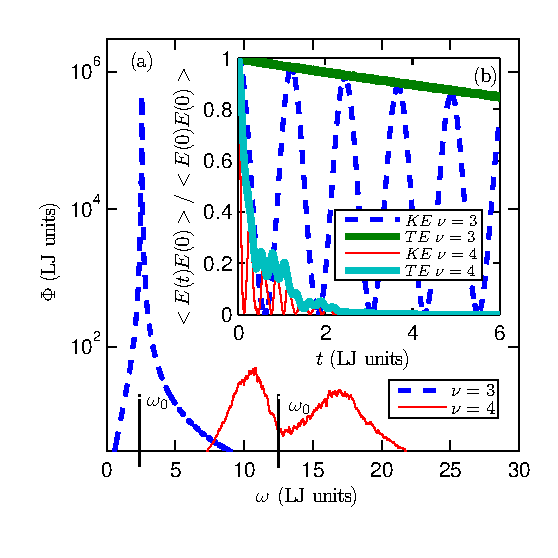
\includegraphics[scale=0.75]
{/home/jason/disorder/lj/alloy/m_lj_nmd_xcorr_compare.eps}
\vspace*{-5mm}
\end{center}
\caption{\label{F:NMD XCORR} The spectral energy density $\Phi$ of 
two modes (polarizations $\nu=3,4$ at wavector [0.2 0 0]) calculated 
using VC-NMD for a mass disordered LJ FCC supercell 
($N_0=8$ and $c=0.5$, Section ). 
The VC dispersion-predicted peaks are labeled 
by $\omega_0$. Inset: the same mode's energy 
(kinetic (KE) and total (TE)) autocorrleation functions.  
Note the additional 
harmonic effects in the KE and TE autoccorelation functions 
for $\nu=4$ which are due to the double peaks in $\Phi$. 
A mode lifetime can 
be extracted unambiguously using the integral of the TE autocorrelation 
function (Section ).}
\end{figure}
%--------------------------------------------------------------------------


%--------------------------------------------------------------------------
\section{\label{A:SF}Calculation of the Gamma Mode Structure Factors}
%--------------------------------------------------------------------------

To calculate 
$S^{L,T}\kw$ for a finite-size system, the 
delta function in Eq. \eqref{EQ:M:SLT} is broadened using a Lorentzian 
function with a full-width at half maximum 
$\Gamma_{FMHW} = \delta_{\omega,avg}$, 
where 
$\delta_{\omega,avg}$ is the average frequency spacing. 
Allen et al\cite{allen_diffusons_1999} 
demonstrated using a model of 
a-Si that the structure factor 
for large wavevector broadens so that the 
linewidth $\Gamma_{SF} > \omega$.
\cite{taraskin_determination_1999}
For the systems sizes studied, $\Gamma_{SF}$ 
scale with the brodening factor 
$\Gamma_{FMHW}$ for all peaks 
except those at high frequencies. 

For the range of broadening factors 
considered ($\Gamma_{FMHW} = \delta_{\omega,avg}$ to $50\delta_{\omega,avg}$) 
the linedwidths extracted for all $c$ 
generally satisfy $\Gamma_{SF} > \omega$. 
For all broadening factors, the linewidths 
(inverse lifetimes, $\tau_{SF} = 1/2\Gamma_{SF}$) 
at high frequency are in better 
agreement with the lifetimes predicted 
by VC-NMD rather than VC-ALD,
where generally $\tau > 2\pi/\omega$ (Ioffe-Refel limit, Fig. ).
\cite{taraskin_determination_1999} This gives a bit more  
justification for the use of the VC predicted group velcoities 
both VC-NMD and VC-ALD, even for large wavevector and $c$. 

In general, the polarization of the eigenvectors $e\kvba$ will not 
be purely transverse or logitudinal along the reciprocal directions. 
Even for the simple LJ argon system, this can make it difficult to 
uniquely identify then different polarizations with the various 
peaks in the structure factors. For SW silicon, similar good agreement 
can be seen along the high symmetry directions for the acoustic branches, 
while the optical modes 
and more complicated polarizations are too difficult to identify in 
an automated way. 
In general, the acoustic branches can be identified, provided they are 
well separated in energy (or frequency) from any optical branches.
\cite{feldman_numerical_1999,thomas_predicting_2010} 

%--------------------------------------------------------------------------
\section{\label{A:Finite Simulation-Size}
Finite Simulation-Size Scaling for Thermal 
Conductivity}
%--------------------------------------------------------------------------
To predict a bulk thermal conductivity, extrapolation is used by the 
following finite size scaling $ 1 / k \propto 1/N_0$. For VC-NMD and 
VC-ALD, the validity of the finite-size scaling 
requires the low frequency modes in the finite system to be dominated by 
intrinsic scattering ($\tau\kv \propto \omega\kv^{-2}$, Section ) and  
follow the Debye approximation 
with respect to $v_{g,\mathbf{n}}$ (Section ) and DOS $D(\omega\kv)$ 
(Section ).\cite{shiomi_thermal_2011,esfarjani_heat_2011} For LJ 
argon, this requirement is satisfied for modest system sizes 
(for $N_0 = 6$ to $12$) so that both VC-NMD and VC-ALD predictions 
can be extrapolated to a bulk value. 
For SW silicon, the thermal conductivity is dominated by low-frequency 
modes (Fig. ). Becasue of this, large system sizes 
(up to $N_0 = 40$) are needed to satsify the 
extrpaolation requirements and only VC-ALD can be used.(cite) This 
demonstrates the computational efficieny of the VC-ALD method which is 
necessary when computationally expensive 
ab initio methods are used (Section ).
\cite{garg_role_2011,tian_phonon_2012,
lindsay_thermal_2012,esfarjani_heat_2011}

System sizes of up to $N_0=38$ are required to predict converged 
thermal conductivity of SW silicon alloys. 
For Si modeled using the Tersoff potential, 
system sizes of up to 64000 atoms are required to observe 
converged values of thermal conductivity using the GK method.
\cite{he_lattice_2012} We find that similar system sizes are 
also required for 

For the GK method, smaller system sizes $N_0 \le 12$ are used for the 
finite size extrapolation for LJ argon and SW silicon . 
The validity of this result can be explained in terms of a 
combination of effects which are specific to the MD simulations.
\cite{esfarjani_heat_2011} In fact, for $c=0$ the GK results are 
independent of system size for $N_0 = 4$ to $N_0 = 12$ for LJ argon.

\clearpage
\bibliographystyle{apsrev}
%\bibliography{/home/jason/sed/jop/asme_prb_paper/prb/references}
\bibliography{/home/jason/Dropbox/ntpl-paper/ntpl-121612}
\end{document}
